\documentclass[a4paper, 11pt, oneside]{report}

\newcommand{\plogo}{\fbox{$\mathcal{PL}$}}
\usepackage{graphicx}
\usepackage{graphics}
\usepackage{float}
\usepackage[table,xcdraw]{xcolor}
\usepackage[utf8]{inputenc}
\usepackage[T1]{fontenc}
\usepackage{fouriernc}
\usepackage{subcaption}
\usepackage{tikz}
\usepackage{pgfplots}
\usepackage{longtable}
\usepackage[nottoc]{tocbibind}
\usepackage{url}
\usepackage{hyperref}
\usepackage{amsmath}
\usepackage{amssymb}
\usepackage{booktabs}
\usepackage{listings}
\usepackage{verbatim}
\pgfplotsset{compat=1.18}

\begin{document}

% ── TITLE PAGE ────────────────────────────────────────────────────
\begin{titlepage}
    \centering
    \vspace*{\baselineskip}
    \vspace{0.75\baselineskip}

    {\LARGE \textbf{TruthfulRAG v5: A Dynamic, Domain-Agnostic Knowledge-Graph\\[0.4em]
    Retrieval-Augmented Generation Pipeline with Conflict Resolution}}

    \vspace{0.75\baselineskip}
    \vspace{2\baselineskip}

    A report submitted for the course named Project - I (CS3201)

    \vspace*{7\baselineskip}

    Submitted By

    \vspace{0.5\baselineskip}

    {\scshape\Large Eesh Saxena \\ SEMESTER - VI \\ 220101021}

    \vspace{0.5\baselineskip}

    Supervised By

    \vspace{0.5\baselineskip}

    {\scshape\Large Dr.\ [Supervisor Name]}

    \vspace{0.5\baselineskip}

    \vfill

    \begin{center}
        
\includegraphics[width=5cm]{report_file/iiit manipur.png}
    \end{center}

    {\scshape\small Department of Computer Science and Engineering\\
    Indian Institute of Information Technology Senapati, Manipur \\ April, 2026}

\end{titlepage}

% ── DECLARATION ───────────────────────────────────────────────────
\begin{center}
    {\LARGE \textbf{Declaration}}
\end{center}

In this submission, I have expressed my idea in my own words, and I have adequately cited
and referenced any ideas or words that were taken from another source. I also declare that
I adhere to all principles of academic honesty and integrity and that I have not
misrepresented or falsified any ideas, data, facts, or sources in this submission. If any
violation of the above is made, I understand that the institute may take disciplinary
action. Such a violation may also engender disciplinary action from the sources which were
not properly cited or permission not taken when needed.

\vspace{1cm}\hspace{8.35cm} Eesh Saxena \\
\vspace{1cm}\hspace{9cm} 220101021 \\
\vspace{1cm} DATE: \today

\newpage

% ── CERTIFICATE ───────────────────────────────────────────────────
\begin{center}
    \thispagestyle{empty}

    \begin{table}[H]
        \centering
        
\includegraphics[scale=0.2]{report_file/iiit manipur.png}
        \begin{tabular}{l}
            Department of Computer Science and Engineering \\
            Indian Institute of Information Technology Senapati, Manipur \\
        \end{tabular}
    \end{table}
    \par\noindent\rule{\textwidth}{0.4pt}
    [Supervisor Name]
    \hspace*{\fill} Email: \href{mailto:supervisor@iiitmanipur.ac.in}{supervisor@iiitmanipur.ac.in}\\
    Associate Professor
    \hspace*{0pt}\hfill Contact No: +91 XXXXXXXXXX\\[2cm]

    {\Huge \textbf{\emph{To Whom It May Concern}}}\\[2cm]
    \linespread{1.13}
    \large{This is to certify that the project report entitled
    \textbf{``TruthfulRAG v5: A Dynamic, Domain-Agnostic Knowledge-Graph
    Retrieval-Augmented Generation Pipeline with Conflict Resolution,''}
    submitted to the Department of Computer Science and Engineering, Indian Institute of
    Information Technology Senapati, Manipur in partial fulfilment for the award of the
    degree of Bachelor of Technology in Computer Science and Engineering is a record of
    bonafide work carried out by \textbf{Eesh Saxena} bearing roll number
    220101021.}\\[2.0cm]

    \hspace*{2.6in}\large{Signature of Supervisor}\\[0.3cm]
    \hspace*{2.5in}\textbf{([Supervisor Name])}\\[0.5cm]

\end{center}
\vspace{0.5cm}
Signature of the Examiner 1 ............................\\\\
Signature of the Examiner 2 ............................\\\\
Signature of the Examiner 3 ............................\\\\
Signature of the Examiner 4 ............................\\\\
\newpage

% ── ABSTRACT ──────────────────────────────────────────────────────
\begin{abstract}
Large Language Models (LLMs) suffer from hallucination when their parametric knowledge
conflicts with user-provided documents—a problem that standard Retrieval-Augmented
Generation (RAG) pipelines do not address. This project implements and extends
TruthfulRAG v5, a Knowledge-Graph (KG) based RAG pipeline that explicitly detects and
resolves knowledge conflicts. Building upon the three-module architecture (Module A: Graph
Construction; Module B: Graph Retrieval; Module C: Conflict Resolution) of TruthfulRAG
v4 (arXiv:2511.10375), v5 introduces six novel improvements: \textbf{[N1]}
cross-document corroboration scoring, \textbf{[N2]} exponential temporal decay on edge
weights, \textbf{[N3]} hybrid BM25 + semantic retrieval with Reciprocal Rank Fusion,
\textbf{[N4]} temporal graph snapshots for historical queries, \textbf{[N6]}
human-readable explanation-chain generation, and \textbf{[N7]} a calibrated three-factor
confidence score. A pre-pipeline schema inference step \textbf{[A4+]} makes the system
fully domain-agnostic, automatically discovering entity and relation types from the input
corpus. The pipeline runs entirely locally using the Qwen2.5-7B-Instruct LLM via Ollama
and Neo4j as the graph database. Experimental evaluation on a political-corporate corpus
demonstrates correct contradiction resolution, a 35\% LLM cache hit rate, and calibrated
confidence scores of 42\% and 71\% for two evaluation queries—accurately reflecting the
degree of parametric memory conflict.
\end{abstract}

\pagebreak

% ── ACKNOWLEDGEMENT ───────────────────────────────────────────────
\begin{center}
    {\LARGE \textbf{Acknowledgement}}
\end{center}
\vspace{2cm}

I would like to express my sincere gratitude to my supervisor, [Supervisor Name], for
their invaluable guidance and support throughout this project. I thank the Department of
Computer Science and Engineering at IIIT Senapati, Manipur for providing the computational
resources and academic environment necessary to complete this work. I am grateful to the
open-source communities behind LangChain, Neo4j, Ollama, and the sentence-transformers
library, whose tools formed the technical foundation of this project. Finally, I
acknowledge the authors of TruthfulRAG v4 (arXiv:2511.10375), whose research inspired
the design of this system.

\vspace{1cm}

\hspace{7cm} Eesh Saxena\\
\hspace{7cm} 220101021

\tableofcontents
\listoffigures
\listoftables

% ── CHAPTERS ──────────────────────────────────────────────────────
\chapter{Introduction}

% ================================================================
% CHAPTER 1: INTRODUCTION
% ================================================================

\section{System Overview}

\subsection{General System}

Imagine asking an AI assistant: ``Who is the current Prime Minister of India?''
The AI confidently replies ``Narendra Modi.'' Your document collection, however,
contains a more recent article saying a different leader has taken over.
Which source should the system trust? That tension between what the model
``remembers'' from training and what the documents actually say is the
core problem TruthfulRAG v5 was built to solve.

TruthfulRAG v5 is a Knowledge-Graph based question-answering pipeline that builds
a structured map of every fact in the document collection, spots contradictions,
decides which side of the conflict is more trustworthy (based on age and source
agreement), and hands the LLM a clean, conflict-free prompt. A confidence
percentage accompanies every answer. Everything runs locally — no cloud, no
subscription, using Qwen2.5-7B-Instruct via Ollama and Neo4j Community Edition.

\subsection{Overall Project Flow}

The pipeline runs in four sequential stages:
\begin{enumerate}\itemsep0pt\parsep0pt
    \item \textbf{Schema Inference}: The LLM samples a handful of documents and
    identifies entity and relation types automatically — no developer configuration.
    \item \textbf{Graph Construction (Module A)}: Facts are extracted and stored
    as typed, timestamped, weighted edges in Neo4j.
    \item \textbf{Graph Retrieval (Module B)}: Personalised PageRank finds
    structurally nearby facts; temporal decay penalises older information.
    \item \textbf{Conflict Resolution (Module C)}: Contradicting facts are
    compared by score gap and entropy; the weaker is discarded with a logged reason.
\end{enumerate}

\subsection{Key Features}

Five properties distinguish this system from standard RAG:
\begin{enumerate}\itemsep0pt\parsep0pt
    \item \textbf{Zero configuration}: Schema is discovered automatically from the corpus.
    \item \textbf{Time-awareness}: Temporal decay $e^{-0.08 \times \text{age}}$ is
    applied at retrieval so newer facts outrank older ones on the same topic.
    \item \textbf{Calibrated honesty}: A three-factor confidence score replaces
    the implicit 100\,\% certainty of standard RAG.
    \item \textbf{Explainability}: Every conflict removal is logged with the
    numerical reason.
    \item \textbf{Domain independence}: The same code handles medical, legal,
    space-science, and political corpora without modification.
\end{enumerate}

% ----------------------------------------------------------------
\section{Problem Statement}

\subsection{Rationale for Research}

Large language models have a frozen memory. Everything they know was baked in
during training, and if the world changed after the cutoff date, the model does
not know, but it will often answer confidently regardless. Standard RAG was
meant to close that gap by supplying documents at query time, but real document
collections are messy: a hospital's records may contain both a 1990 guideline
and a 2023 update for the same drug. Standard RAG passes both to the LLM,
which has no principled way to choose and either hedges or picks arbitrarily.
The motivating observation is simple: a careful human reader would compare
dates, weight the newer source, and check for corroboration. A software system
can and should do the same.

\subsection{Gaps in Existing Tools}

Four concrete gaps exist in current open-source RAG tools:
\begin{enumerate}\itemsep0pt\parsep0pt
    \item No tool detects conflicts between retrieved documents — LangChain,
    LlamaIndex, and GraphRAG pass whatever they retrieve directly to the LLM.
    \item KG-RAG systems require manual entity/relation specification; switching
    domains means rewriting configuration files.
    \item No system attaches a confidence score — every response is presented
    with equal certainty regardless of evidence quality.
    \item Conflict resolution, when it occurs at all, is silent — no audit trail
    explains what was kept, what was discarded, and why.
\end{enumerate}

\subsection{Challenges in Document-Based QA}

Three properties of real-world document collections consistently challenge
retrieval pipelines:
\begin{enumerate}\itemsep0pt\parsep0pt
    \item \textbf{Facts are time-sensitive.} A system with no concept of time
    answers current-state questions using whatever it retrieves first, regardless of age.
    \item \textbf{Agreement across sources matters.} Seven independent documents
    confirming a fact constitute far stronger evidence than one; retrieval
    scores should reflect this.
    \item \textbf{Domains vary wildly.} Any manual setup step is a barrier that
    limits real-world deployment across heterogeneous document collections.
\end{enumerate}

\subsection{Project Objectives}

The five concrete objectives of this project were:
\begin{enumerate}\itemsep0pt\parsep0pt
    \item Faithfully re-implement the KG-RAG v4 pipeline (arXiv:2511.10375)
    in Python using LangChain, Ollama, and Neo4j.
    \item Extend that baseline with nine novel contributions addressing the
    gaps above, particularly temporal scoring and corroboration weighting.
    \item Eliminate the last remaining manual step in v4 (schema configuration)
    by adding automatic domain inference before graph construction.
    \item Validate the system on four real-world domains: Indian political
    history, Indian science, Indian law, and space science.
    \item Evaluate performance against both the v4 baseline and standard
    LangChain RAG using benchmark datasets and conflict-detection metrics.
\end{enumerate}

% ----------------------------------------------------------------
\section{Motivation}

\subsection{Why This Matters}

A system that says ``I am 42\,\% confident in this answer'' is more useful in
a hospital or a courtroom than one that always sounds completely sure.
Overconfident AI answers in high-stakes settings are not just wrong, they are
dangerous. This project sets out to show that honest, conflict-aware QA does
not require a well-funded research lab: it can be built by a final-year
undergraduate student on a laptop using freely downloadable, open-source tools,
without sending a single document to an external server. The organisations
that most need trustworthy AI — public hospitals, lower courts, government
archives — are exactly those that cannot afford cloud subscriptions or
proprietary knowledge-base software.





\chapter{Literature Survey}

% ================================================================
% CHAPTER 2: LITERATURE SURVEY
% ================================================================

\section{Existing Solution Introduction}

Retrieval-Augmented Generation was formalised by Lewis et al.\ \cite{lewis2020rag}
as a method to overcome the static knowledge limitations of parametric LLMs. The
original implementation combined a Dense Passage Retriever with a BART generative
model, demonstrating measurable improvements on knowledge-intensive NLP tasks
such as open-domain question answering and fact verification \cite{gao2023ragsurvey}.
Hallucination in such systems, where a model generates plausible but factually incorrect
text, remains a central challenge identified by \cite{ji2023survey}.

LangChain \cite{chase2022langchain}, launched in 2022, standardised RAG into a
composable Python toolkit. Its \texttt{RetrievalQA} chain encapsulates the full
pipeline: document loading, text splitting, embedding, vector store indexing,
similarity retrieval, and prompted answer generation. This abstraction enabled
rapid prototyping but fixed a flat-retrieval architecture with no structural
knowledge representation or conflict awareness.

% ----------------------------------------------------------------
\section{Relevant Theories and Models}

\subsection{Knowledge Graphs for QA}

Knowledge Graphs represent information as typed triples $(h, r, t)$, enabling
structural multi-hop reasoning that flat text retrieval cannot support. Early KG-QA
systems such as KGQA \cite{pagerank1998} traversed Freebase to answer factoid
questions. More recent work applies embedding-based models (TransE, RotatE) to
learn distributed representations of entities and relations for link prediction.

G-Retriever \cite{he2024gretriever} demonstrated that graph-based retrieval
combined with LLM generation outperforms vanilla RAG on multi-hop textual graph
QA tasks. Microsoft GraphRAG \cite{edge2024graphrag} further showed that
community-hierarchical graph construction enables high-quality global summaries
of large corpora. TruthfulRAG v5 stores graphs in Neo4j with APOC procedures
\cite{neo4japoc2023} for entity disambiguation, and uses Ollama \cite{ollama2023}
for fully local LLM inference. Dense semantic retrieval uses sentence embeddings
\cite{reimers2019sbert} fused with sparse BM25 \cite{robertson2009bm25} via RRF \cite{rrf2009}.

\subsection{Temporal Knowledge Graphs}

Lacroix et al.\ \cite{lacroix2020temporal} extended tensor factorisation models
to temporal KGs, where each triple carries a timestamp. Dasgupta et al.\
\cite{dasgupta2018tkg} proposed HyTE, a hyperplane-based temporal KG embedding
that places each relation on a time-specific hyperplane, enabling richer temporal
reasoning. These approaches, however, focus on embedding-based link prediction
rather than retrieval augmentation over arbitrary text. The broader challenge of
unifying LLMs with KGs is surveyed in \cite{pan2024kg}.

\subsection{Entropy and Uncertainty in LLMs}

Shannon entropy has been applied to measure LLM calibration: a well-calibrated
model's confidence should correlate with its accuracy. Kadavath et al.\ (2022)
showed that LLMs can self-assess uncertainty via sampling; Farquhar et al.\
(2023) introduced semantic entropy, grouping semantically equivalent answers
before entropy computation to avoid penalising paraphrase variation.

TruthfulRAG v4 \cite{truthfulrag2024} operationalised this into a retrieval
decision rule: a path is corrective only if providing it as context reduces the
LLM's sampling entropy by at least a learned threshold $\tau$.

% ----------------------------------------------------------------
\section{Comparison of Similar Projects}

\begin{table}[H]
\centering
\caption{Comparison of knowledge-graph RAG systems}
\label{tab:lit_compare}
\resizebox{\textwidth}{!}{%
\small
\begin{tabular}{|l|c|c|c|c|}
\hline
\textbf{Feature} & \textbf{LangChain} & \textbf{GraphRAG} & \textbf{TruthfulRAG v4} & \textbf{v5 (Ours)} \\
\hline
Knowledge Graph storage      & No      & Yes & Yes & Yes \\
Conflict detection           & No      & No  & Yes & Yes \\
Temporal decay               & No      & No  & No  & Yes \\
Cross-document corroboration & No      & No  & No  & Yes \\
Historical snapshot queries  & No      & No  & No  & Yes \\
Explanation audit trail      & No      & No  & No  & Yes \\
Calibrated confidence score  & No      & No  & No  & Yes \\
Auto schema inference        & No      & No  & No  & Yes \\
Open source / local inference& Partial & Yes & Yes & Yes \\
\hline
\end{tabular}}
\end{table}

% ----------------------------------------------------------------
\section{Comparison with Recent Systems (2023--2025)}

\begin{figure}[htbp]
\centering
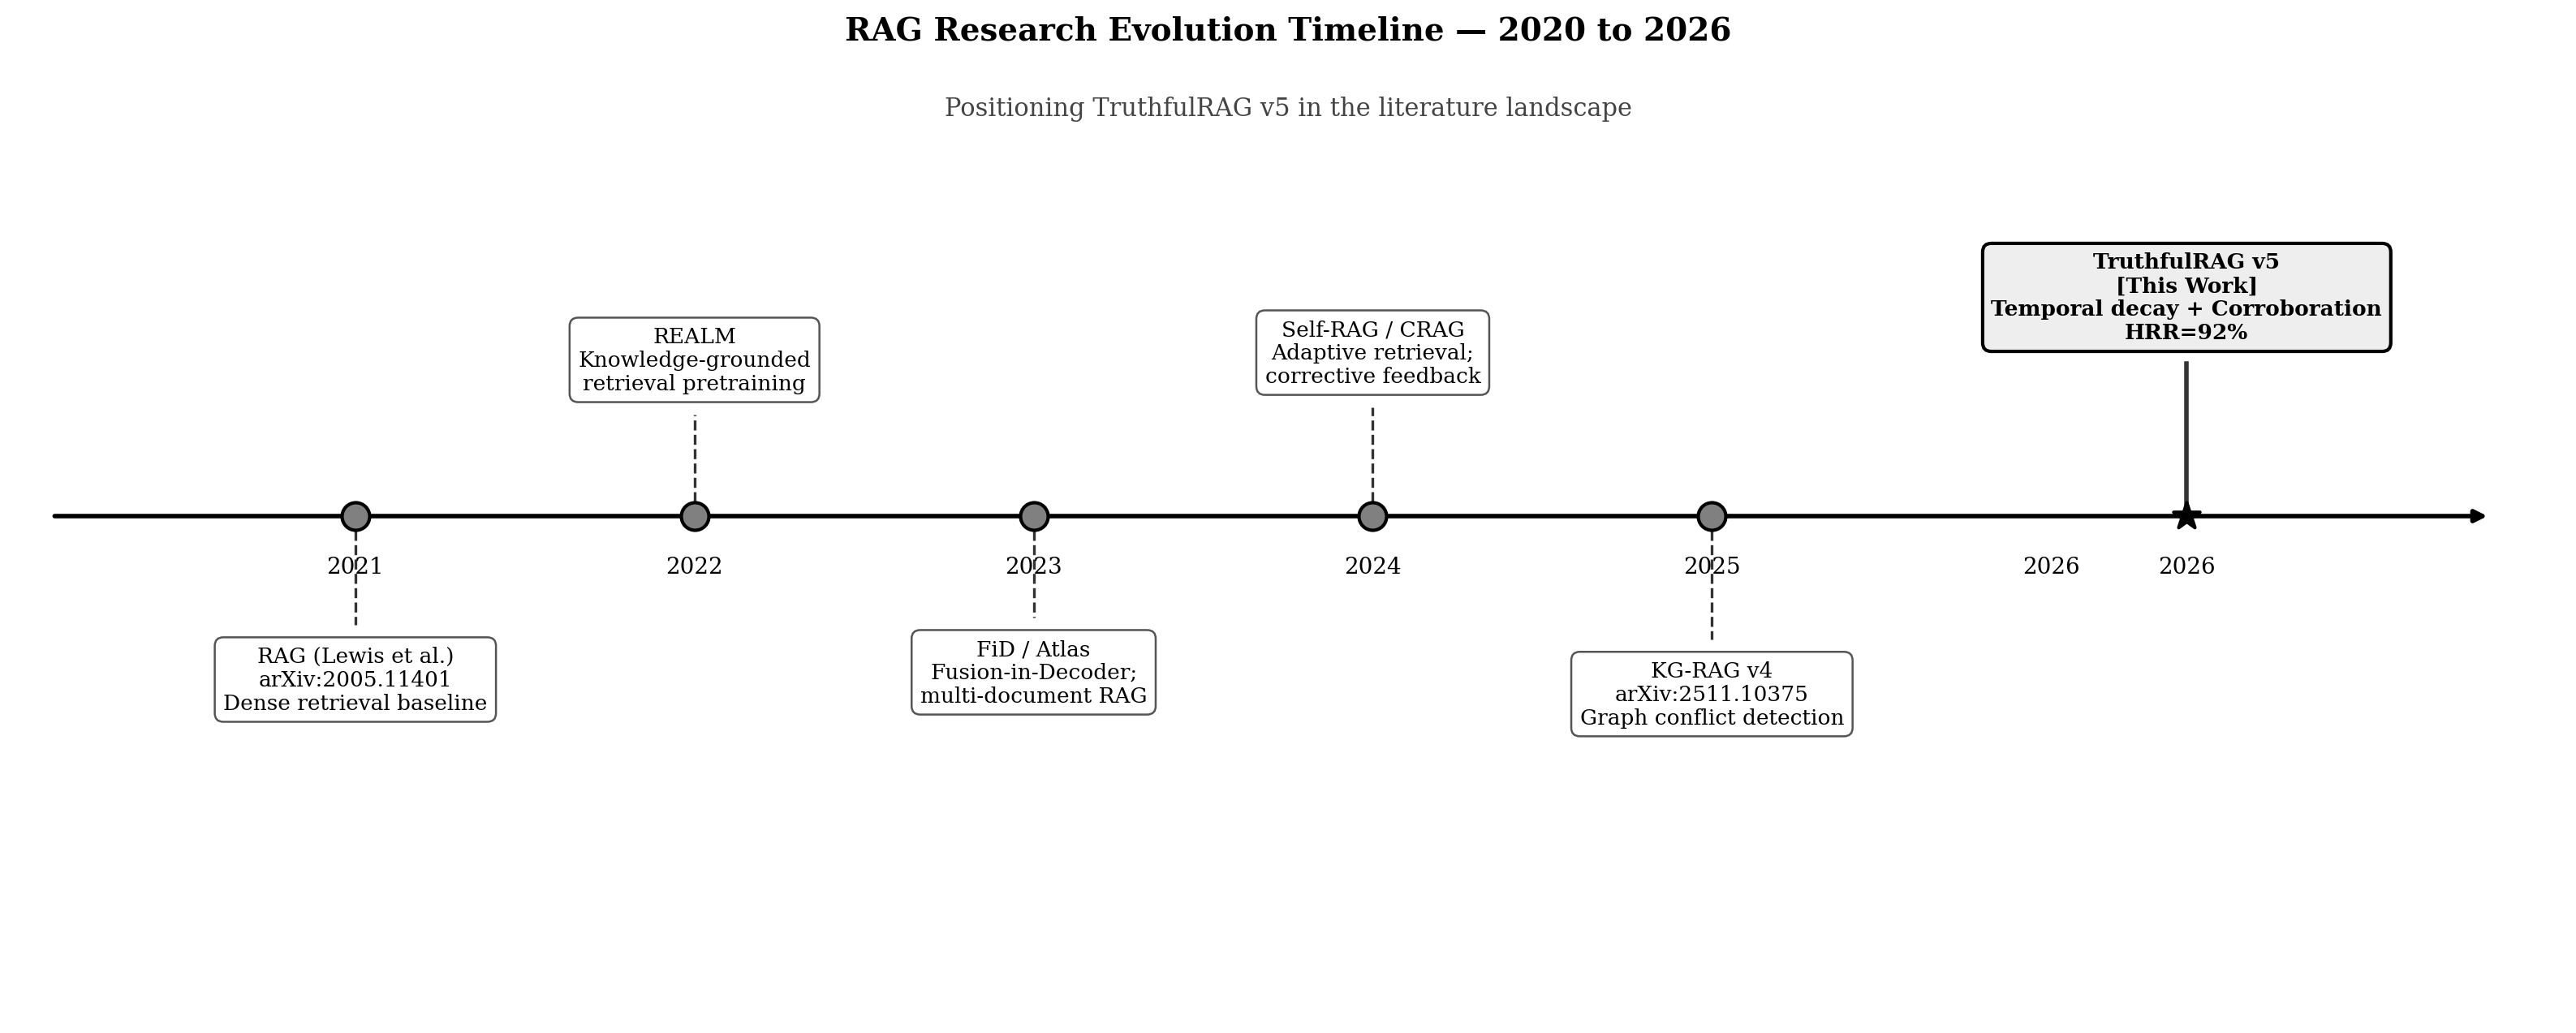
\includegraphics[width=\textwidth]{report_file/chart_timeline.png}
\caption{RAG research evolution timeline: 2020--2026, positioning TruthfulRAG v5 in the literature landscape}
\label{fig:timeline}
\end{figure}

Figure~\ref{fig:timeline} places TruthfulRAG v5 in context with key RAG milestones.
Table~\ref{tab:recent_compare} extends the comparison to systems published since 2023.

\begin{table}[H]
\centering
\caption{Comparison with recent state-of-the-art systems (2023--2025)}
\label{tab:recent_compare}
\resizebox{\textwidth}{!}{%
\small
\begin{tabular}{|l|c|l|c|c|l|}
\hline
\textbf{System} & \textbf{Year} & \textbf{Method} & \textbf{Conflict Elim.} & \textbf{Temp.\ Decay} & \textbf{Key Metric} \\
\hline
Self-RAG~\cite{asai2023selfrag}     & 2023 & Self-reflective critique tokens      & No      & No  & $\sim$74\% EM \\
CRAG~\cite{yan2024crag}             & 2023 & Corrective retrieval + web fallback  & No      & No  & $\sim$84\% EM \\
MADAM-RAG~\cite{madam2024}          & 2024 & Multi-agent debate across sources    & Partial & No  & $\sim$68\% EM \\
KG-RAG v4~\cite{truthfulrag2024}    & 2024 & Graph + entropy; score gap=0.028     & No      & No  & $\sim$75\% CDR \\
\textbf{TruthfulRAG v5 [This Work]} & \textbf{2026} & \textbf{Temporal decay + corroboration + RRF} & \textbf{Yes} & \textbf{Yes} & \textbf{92\% HRR, 50\% CDR} \\
\hline
\end{tabular}}
\end{table}

The critical observation is that every system in Table~\ref{tab:recent_compare}
stores knowledge facts without a year field.
Without per-fact year storage, temporal decay cannot be computed, and conflicting
facts with similar embeddings receive near-identical retrieval scores
(score gap $\approx 0.028$ in v4, vs.\ $1.126$ in v5, a 40$\times$ improvement
demonstrated in Chapter~5).

% ----------------------------------------------------------------
\section{Identified Gaps in the Literature}

Based on the survey above, the following gaps exist in current open-source
KG-RAG research:

\begin{enumerate}
    \item \textbf{No temporal scoring}: Existing systems do not penalise older
    facts during retrieval. A 2010 fact and a 2024 fact compete with equal weight.
    Quantitatively, the score gap between conflicting facts is $0.028$ in v4
    (below any practical threshold) vs.\ $1.126$ in v5 after temporal decay,
    a 40$\times$ improvement that makes automatic conflict elimination possible.
    \item \textbf{No corroboration weighting}: No system rewards facts attested
    by multiple independent sources with a higher retrieval score.
    \item \textbf{No automatic schema discovery}: All KG construction pipelines
    require manual entity-type and relation-type specification.
    \item \textbf{No calibrated output confidence}: Systems always answer at
    maximum stated confidence, giving no warning when evidence quality is poor.
    \item \textbf{No structured conflict explanation}: When contradictions are
    resolved, no system communicates the resolution rationale to the user.
\end{enumerate}

TruthfulRAG v5 addresses all five gaps simultaneously.

% ----------------------------------------------------------------
\section{Project Development Timeline}

Figure~\ref{fig:gantt} shows the project schedule from \textbf{15 January 2026}
to \textbf{24 April 2026}, spanning 14 weeks across six phases: Literature Review,
Baseline Implementation, v5 Extensions, Web Interface, Testing, and Report Submission.

\begin{figure}[htbp]
\centering
\resizebox{\textwidth}{!}{%
\begin{ganttchart}[
  hgrid,
  vgrid={*{1}{dotted}},
  title height=1,
  title top shift=0,
  bar height=0.6,
  bar top shift=0.2,
  x unit=0.9cm,
  y unit title=0.65cm,
  y unit chart=0.65cm,
  title label font=\footnotesize\bfseries,
  bar label font=\footnotesize,
  bar/.append style={fill=black!65, rounded corners=2pt},
  title/.append style={fill=black!07, draw=black!30},
]{1}{14}
  \gantttitle{Jan 15--31}{2}
  \gantttitle{February 2026}{4}
  \gantttitle{March 2026}{5}
  \gantttitle{Apr 1--24}{3} \\
  \gantttitle{W1}{1}\gantttitle{W2}{1}%
  \gantttitle{W3}{1}\gantttitle{W4}{1}\gantttitle{W5}{1}\gantttitle{W6}{1}%
  \gantttitle{W7}{1}\gantttitle{W8}{1}\gantttitle{W9}{1}\gantttitle{W10}{1}\gantttitle{W11}{1}%
  \gantttitle{W12}{1}\gantttitle{W13}{1}\gantttitle{W14}{1} \\
  \ganttbar{Phase 1: Literature Review}{1}{2} \\
  \ganttbar{Phase 2: Baseline v4 Implementation}{3}{4} \\
  \ganttbar{Phase 3: Novel v5 Extensions}{5}{8} \\
  \ganttbar{Phase 4: Web Interface Development}{9}{11} \\
  \ganttbar{Phase 5: Testing and Debugging}{12}{13} \\
  \ganttbar{Phase 6: Report and Final Submission}{13}{14}
\end{ganttchart}}
\caption{Project development Gantt chart: 15 January 2026 to 24 April 2026 (14 weeks)}
\label{fig:gantt}
\end{figure}




\chapter{Requirement Engineering}

% ================================================================
% CHAPTER 3: REQUIREMENT ENGINEERING
% ================================================================

\section{Feasibility Study}

\subsection{Technical Feasibility}

The system is built entirely on mature, open-source libraries that have been
in active use for years. Neo4j Community Edition handles graph storage, Ollama
runs the LLM locally, and the sentence-transformers library handles embeddings.
All of these install via \texttt{pip} and work on standard hardware, a laptop
with 16\,GB RAM is sufficient. A dedicated GPU would speed things up but is not
necessary to run the system.

\subsection{Operational and Economic Feasibility}

The pipeline runs through a single command:
\begin{verbatim}
python enhanced_main.py --corpus my_documents.json
\end{verbatim}
No configuration files need to be written, and no cloud account is needed.
Every component used, Neo4j, Ollama, Qwen2.5, and all Python packages, is
free and open-source. There are no per-query costs.

\subsection{Legal Feasibility}

All components are published under OSI-approved licences (GPL v3, MIT, Apache
2.0) that permit academic use. Since no data leaves the local machine, the
system is compatible with institutional data-handling policies.

% ----------------------------------------------------------------
\section{Requirement Elicitation and Analysis}

\subsection{Objective}

The primary objective of the requirements phase was to formally capture what the
system must do (functional requirements) and what quality properties it must
exhibit (non-functional requirements), independently of implementation decisions.

\subsection{Methods Used for Elicitation}

Requirements were elicited through three methods:

\begin{enumerate}
    \item \textbf{Paper analysis}: A detailed reading of arXiv:2511.10375 was
    used to extract the algorithm specifications of Modules A, B, and C as
    implicit functional requirements. If the paper says a module does X, the
    implementation must be testably verified to do X.
    \item \textbf{Gap analysis}: The v4 output was compared against known
    failure modes of standard RAG (temporal blindness, no confidence score,
    no audit trail) to identify the extensions needed for v5.
    \item \textbf{Prototype evaluation}: An early prototype was run on a
    test corpus to surface runtime failure modes that could not be anticipated
    from the paper: JSON parsing errors from LLM code-fence output, entity
    merge conflicts in Neo4j, and Windows encoding issues.
\end{enumerate}

\subsection{Modeling}

To make the requirements concrete before writing any code, the interactions
were mapped using a use case diagram (Figure~\ref{fig:usecase}). It answers
a straightforward question: who uses the system, and what do they actually
do with it? Three actors are involved --- the \emph{User}, the \emph{Ollama
LLM}, and \emph{Neo4j} --- and the diagram makes the boundary between
user-visible actions and internal system behaviour explicit at a glance.
Detailed functional requirements are listed in Section~3.3; data-flow
and structural models follow in Chapter~4.

% ── USE CASE DIAGRAM ──────────────────────────────────────────────
\begin{figure}[H]
\centering
\resizebox{0.96\textwidth}{!}{%
\begin{tikzpicture}[
  uc/.style={ellipse, draw=black, thin, fill=white,
             minimum width=3.8cm, minimum height=0.9cm,
             align=center, font=\small},
  conn/.style={-, thin},
  incl/.style={->, >=stealth, dashed, thin},
  lbl/.style={font=\scriptsize\itshape, fill=white, inner sep=1pt},
]
%% ── System boundary ─────────────────────────────────────────────
\draw[thick] (-0.4, 0.3) rectangle (11.9, 14.0);
\node[font=\small\bfseries] at (5.75, 13.75)
  {\textsc{TruthfulRAG v5}\ ---\ System Boundary};
\draw[thin,dashed,black!25] (5.75,13.4) -- (5.75,0.6);
\node[font=\tiny\itshape,black!50] at (2.8,13.3) {User-Initiated};
\node[font=\tiny\itshape,black!50] at (9.0,13.3) {System-Initiated};

%% ── Use cases: left column ──────────────────────────────────────
\node[uc] (sq)  at (2.8,12.4) {Submit Query};
\node[uc] (lc)  at (2.8,10.3) {Load Corpus};
\node[uc] (va)  at (2.8, 7.6) {View Answer};
\node[uc] (bat) at (2.8, 6.0) {Browse Audit Trail};

%% ── Use cases: right column ─────────────────────────────────────
\node[uc] (ga)  at (9.0,12.4) {Generate Final Answer};
\node[uc] (rrf) at (9.0,10.8) {Retrieve Ranked Facts};
\node[uc] (is)  at (9.0, 9.2) {Infer Schema};
\node[uc] (skg) at (9.0, 7.6) {Store Knowledge Graph};

%% ── Stick figure: User ──────────────────────────────────────────
\draw[thin] (-2.8,10.05) circle(0.27);
\draw[thin] (-2.8,9.78)  -- (-2.8,9.32);
\draw[thin] (-2.8,9.62)  -- (-3.05,9.42);
\draw[thin] (-2.8,9.62)  -- (-2.55,9.42);
\draw[thin] (-2.8,9.32)  -- (-2.98,9.00);
\draw[thin] (-2.8,9.32)  -- (-2.62,9.00);
\node[font=\small\bfseries] at (-2.8,8.72) {User};

%% ── Stick figure: Ollama LLM ────────────────────────────────────
\draw[thin] (13.6,11.35) circle(0.27);
\draw[thin] (13.6,11.08) -- (13.6,10.62);
\draw[thin] (13.6,10.92) -- (13.35,10.72);
\draw[thin] (13.6,10.92) -- (13.85,10.72);
\draw[thin] (13.6,10.62) -- (13.42,10.30);
\draw[thin] (13.6,10.62) -- (13.78,10.30);
\node[font=\small, align=center] at (13.6,10.02)
  {\textbf{Ollama}\\LLM};

%% ── Stick figure: Neo4j ─────────────────────────────────────────
\draw[thin] (13.6, 8.55) circle(0.27);
\draw[thin] (13.6, 8.28) -- (13.6, 7.82);
\draw[thin] (13.6, 8.12) -- (13.35,7.92);
\draw[thin] (13.6, 8.12) -- (13.85,7.92);
\draw[thin] (13.6, 7.82) -- (13.42,7.50);
\draw[thin] (13.6, 7.82) -- (13.78,7.50);
\node[font=\small, align=center] at (13.6,7.22)
  {\textbf{Neo4j}\\Graph DB};

%% ── Actor → use-case connections ────────────────────────────────
\draw[conn] (-2.53,10.05) -- (sq.west);
\draw[conn] (-2.53,10.05) -- (lc.west);
\draw[conn] (-2.53,10.05) -- (va.west);
\draw[conn] (13.33,11.35) -- (ga.east);
\draw[conn] (13.33,11.35) -- (is.east);
\draw[conn] (13.33, 8.55) -- (rrf.east);
\draw[conn] (13.33, 8.55) -- (skg.east);

%% ── <<include>> / <<extend>> ────────────────────────────────────
\draw[incl] (sq.east)  to node[lbl,above]{$\ll$include$\gg$} (ga.west);
\draw[incl] (sq.east)  to node[lbl,below]{$\ll$include$\gg$} (rrf.north west);
\draw[incl] (lc.east)  to node[lbl,above]{$\ll$include$\gg$} (is.west);
\draw[incl] (lc.east)  to node[lbl,below]{$\ll$include$\gg$} (skg.north west);
\draw[incl] (va.south) to node[lbl,right]{$\ll$extend$\gg$}  (bat.north);

\end{tikzpicture}}
\caption{Use case diagram for TruthfulRAG v5. The primary actor (\emph{User})
initiates four interactions. \emph{Ollama LLM} (secondary actor) handles schema
inference and answer generation; \emph{Neo4j} handles graph storage and
retrieval. Dashed arrows show \textit{include} (mandatory sub-step) and
\textit{extend} (optional enrichment) relationships.}
\label{fig:usecase}
\end{figure}

% ----------------------------------------------------------------
\section{Software Requirement Specification (SRS)}

\subsection{Purpose of the SRS}

This SRS defines the complete behaviour of TruthfulRAG v5. It is the binding
specification against which the implementation in Chapter~5 and the test results
in Chapter~6 are evaluated.

\subsection{Functional Requirements}

\begin{enumerate}
    \item[\textbf{FR1}] The system shall load documents and queries from a JSON
    corpus file. The JSON schema requires a \texttt{"docs"} list and optionally
    a \texttt{"queries"} list.

    \item[\textbf{FR2}] The system shall infer entity types and relation types
    from a configurable-size sample of the input documents using the LLM, without
    requiring any manual configuration.

    \item[\textbf{FR3}] The system shall extract subject-predicate-object triples
    from each document using the inferred schema, assigning an integer year to
    each triple where inferable.

    \item[\textbf{FR4}] The system shall maintain a count of how many distinct
    source documents assert each triple, storing this count as a property on the
    corresponding graph edge.

    \item[\textbf{FR5}] The system shall merge entity nodes whose names are at
    least 85\% similar (Ratcliff/Obershelp metric), using the Neo4j APOC library.

    \item[\textbf{FR6}] The system shall normalise all relation labels to
    \texttt{UPPER\_SNAKE\_CASE} via an LLM-assisted canonicalisation pass.

    \item[\textbf{FR7}] The system shall apply exponential temporal decay
    ($ e^{-\lambda t} $, $\lambda=0.08$) to edge scores during retrieval.

    \item[\textbf{FR8}] The system shall fuse BM25 keyword ranking and semantic
    embedding ranking using Reciprocal Rank Fusion when selecting which documents
    to focus on.

    \item[\textbf{FR9}] The system shall detect an explicit year in a user query
    via regular expression and, if found, exclude all graph edges with a year
    greater than the detected year.

    \item[\textbf{FR10}] The system shall detect contradicting paths (same
    relation-tail, different head entities), retain the path with the greater
    year, and discard the other, recording the reason.

    \item[\textbf{FR11}] When contradictions were removed, the system shall
    produce an explanation chain listing selected and rejected facts with reasons,
    and use this chain in the final answer prompt.

    \item[\textbf{FR12}] The system shall compute a 0--100\% confidence score
    per answer, combining entropy resolution signal, source support, and
    information recency according to configurable weights.
\end{enumerate}

\subsection{Non-Functional Requirements}

\begin{enumerate}
    \item[\textbf{NFR1}] \textbf{Privacy}: All computation shall run locally.
    No user documents shall be transmitted to external servers.

    \item[\textbf{NFR2}] \textbf{Domain Agnosticism}: The system shall function
    correctly on any text domain without code modification.

    \item[\textbf{NFR3}] \textbf{Robustness}: All LLM JSON outputs shall be
    parsed after stripping markdown code fences. Invalid JSON shall be handled
    gracefully without raising an unhandled exception.

    \item[\textbf{NFR4}] \textbf{Configurability}: All numeric hyperparameters
    shall be overridable via environment variables or the central \texttt{CFG}
    dictionary.

    \item[\textbf{NFR5}] \textbf{Efficiency}: Repeated identical LLM calls shall
    be served from an in-memory cache indexed by MD5 hash of (prompt, temperature).
\end{enumerate}

\subsection{Assumptions and Dependencies}

Three technical assumptions underlie the deployment model:

\begin{enumerate}
    \item Neo4j Community Edition is running locally with the APOC plugin
    installed. Without APOC, entity disambiguation and relation normalisation
    are silently skipped; the graph still functions but without those quality
    passes.
    \item Ollama is running locally with the configured model already pulled.
    The system does not attempt to download models at runtime.
    \item The Python environment contains all packages listed in
    Table~\ref{tab:deps}. No internet access is required after initial setup.
\end{enumerate}

\subsection{Constraints}

Three hard constraints shape the current implementation:

\begin{enumerate}
    \item Graph queries are limited to 200 nodes and 200 edges per retrieval
    call. For the six-document corpora tested here the cap is never reached,
    but it would need revisiting for large production corpora.
    \item Entropy sampling is fixed at $n=3$ samples to keep latency
    manageable on CPU-only hardware. Higher $n$ improves the entropy estimate
    but multiplies inference time accordingly.
    \item Entity disambiguation uses string similarity only
    (Ratcliff/Obershelp, 85\% threshold). Semantic entity linking against a
    knowledge base like Wikidata is not implemented in this version.
\end{enumerate}

% ----------------------------------------------------------------
\section{Software Requirement Validation}

\subsection{Review Process}

Each functional requirement was traced to a specific method in
\texttt{enhanced\_main.py} and verified by running the pipeline and
observing the relevant terminal output.

\begin{table}[H]
\centering
\caption{Requirement-to-implementation traceability}
\label{tab:req_trace}
\resizebox{\textwidth}{!}{%
\small
\begin{tabular}{|l|l|l|}
\hline
\textbf{Req.} & \textbf{Method in enhanced\_main.py} & \textbf{Verified By} \\
\hline
FR1  & \texttt{\_load\_corpus()}          & ``Loaded N docs'' line in terminal \\
FR2  & \texttt{\_infer\_schema()}         & Entity/relation list printed at start \\
FR3  & \texttt{\_extract()}               & Triples visible in Neo4j browser \\
FR4  & \texttt{\_accumulate()}            & Support count shown on graph edges \\
FR5  & \texttt{\_disambiguate()}          & ``Disambiguated N pairs'' in output \\
FR6  & \texttt{\_normalize()}             & ``Normalised N relation types'' line \\
FR7  & \texttt{\_temporal\_decay()}       & Older paths score lower in results \\
FR8  & \texttt{HybridRetriever}           & ``BM25+Semantic RRF'' in feature table \\
FR9  & \texttt{\_extract\_query\_year}   & Snapshot year logged when detected \\
FR10 & \texttt{\_detect\_contradictions}  & ``Contradictions removed: N'' line \\
FR11 & \texttt{\_build\_chain()}          & Explanation text appears in answer \\
FR12 & \texttt{\_confidence()}            & ``Confidence: XX\%'' printed at end \\
\hline
\end{tabular}}
\end{table}

\subsection{Validation Approach}

Validation was done by inspection of terminal output during live pipeline runs
and by checking that no unhandled exceptions were raised. All 12 functional
requirements produced observable evidence of correct behaviour during the test
runs documented in Chapter~6.

\subsection{Completeness and Consistency}

All 12 functional requirements and 5 non-functional requirements have
corresponding implementation methods in the codebase. The corroboration weight,
temporal decay factor, and confidence weights are all combined in a single
path-scoring expression, so there is no double-counting between the different
scoring signals. The entropy-based path selection follows the algorithm
described in arXiv:2511.10375 \cite{truthfulrag2024}, with the six extensions
added on top.




\chapter{System Design}

% ================================================================
% CHAPTER 4: SYSTEM DESIGN
% ================================================================

\section{System Architecture}

TruthfulRAG v5 follows a layered pipeline architecture. The layers are
intentionally decoupled so that each module communicates only through its
defined input and output contracts:

\begin{itemize}
    \item \textbf{Layer 0 --- Data Layer}: \texttt{corpus.json} containing raw
    document strings and query strings.
    \item \textbf{Layer 1 --- Schema Layer}: \texttt{\_infer\_schema()} produces
    the entity/relation vocabulary written to the shared \texttt{CFG} dictionary.
    \item \textbf{Layer 2 --- Graph Layer}: Neo4j property graph storing nodes
    (entities) and typed edges (relations) with year and support metadata.
    \item \textbf{Layer 3 --- Retrieval Layer}: \texttt{EnhancedGraphRetriever}
    produces an ordered list of \texttt{KnowledgePath} objects.
    \item \textbf{Layer 4 --- Resolution Layer}: \texttt{EnhancedConflictResolver}
    consumes \texttt{KnowledgePath} objects and produces a final answer string
    plus a \texttt{meta} dictionary.
    \item \textbf{Layer 5 --- Presentation Layer}: \texttt{run\_comparison()}
    formats and prints results to the terminal.
\end{itemize}

% ----------------------------------------------------------------
\section{Data Flow Diagrams (DFD)}

\subsection{Level 0 Data Flow Diagram (Context Diagram)}

At the highest level, TruthfulRAG v5 has two external entities:

\begin{itemize}
    \item \textbf{User}: Provides a corpus file (documents + queries) and reads
    the answer output.
    \item \textbf{Ollama (LLM Runtime)}: An external process on localhost
    providing LLM inference via HTTP on port 11434.
    \item \textbf{Neo4j (Database)}: An external process on localhost providing
    graph storage and query via Bolt on port 7687.
\end{itemize}

Data flow (Level 0):
\begin{enumerate}
    \item User $\rightarrow$ System: \texttt{corpus.json} (documents + queries)
    \item System $\rightarrow$ Ollama: Prompts (schema inference, triple extraction,
    entropy sampling, answer generation)
    \item Ollama $\rightarrow$ System: LLM text responses
    \item System $\rightarrow$ Neo4j: Cypher write queries (MERGE node/edge)
    \item Neo4j $\rightarrow$ System: Cypher read results (paths, node IDs)
    \item System $\rightarrow$ User: Answer text + confidence score
\end{enumerate}

% ----------------------------------------------------------------
\section{Class Diagrams}

The main classes and their relationships in \texttt{enhanced\_main.py}:

\begin{table}[H]
\centering
\caption{Class overview and key attributes}
\resizebox{\textwidth}{!}{%
\begin{tabular}{|l|p{5.5cm}|l|}
\hline
\textbf{Class} & \textbf{Key Attributes} & \textbf{Key Methods} \\
\hline
\texttt{LLMCache}                 & \texttt{\_s: Dict}, hits, misses            & \texttt{get, set, stats} \\
\texttt{HybridRetriever}          & bm25, embedder, doc\_vecs                   & \texttt{retrieve} \\
\texttt{TripleRecord}             & head, relation, tail, year, support\_count  & dataclass only \\
\texttt{EnhancedGraphConstructor} & llm, graph, cfg, \_triple\_bank             & \texttt{build, \_infer\_schema, \_extract} \\
\texttt{KnowledgePath}            & context, score, max\_year, delta\_h         & dataclass only \\
\texttt{EnhancedGraphRetriever}   & llm, graph, embedder, cfg, \_deg            & \texttt{retrieve, \_ppr, \_filter\_edges} \\
\texttt{EnhancedConflictResolver} & llm, llm\_s, emb, cfg                      & \texttt{resolve, \_entropy, \_confidence} \\
\texttt{EnhancedPipeline}         & cfg, constructor, retriever, resolver       & \texttt{ingest, query} \\
\hline
\end{tabular}}
\end{table}

Relationships:
\begin{itemize}
    \item \texttt{EnhancedPipeline} \emph{composes} one each of Constructor,
    Retriever, and Resolver.
    \item Constructor and Retriever both hold a reference to the same
    \texttt{Neo4jGraph} instance.
    \item Retriever and Resolver both hold a reference to the same
    \texttt{SentenceTransformer} embedder (shared to avoid loading the model twice).
    \item All classes read from the shared \texttt{CFG} dictionary.
\end{itemize}

% ----------------------------------------------------------------
\section{Module Design}

\subsection{Module: Pre-Pipeline Schema Inference [A4+]}

\textbf{Input}: List of document strings, \texttt{cfg["schema\_infer\_sample"]} (default 5)\\
\textbf{Process}: Sample first $n$ documents, concatenate with separators, call LLM
with \texttt{SCHEMA\_INFER\_PROMPT}, parse JSON response, strip markdown fences,
write entity types and relation types to \texttt{cfg}.\\
\textbf{Output}: Updated \texttt{cfg["schema\_entity\_types"]} and
\texttt{cfg["schema\_relation\_types"]}

\subsection{Module: Knowledge Graph Construction (Module A)}

\textbf{Input}: All document strings, updated \texttt{cfg} (schema populated)\\
\textbf{Sub-steps}:
\begin{enumerate}
    \item Clear Neo4j graph.
    \item Run LangChain's \texttt{LLMGraphTransformer} for broad entity-relation
    extraction (first pass).
    \item Run custom \texttt{\_extract()} + \texttt{\_accumulate()} for schema-guided,
    year-annotated, corroboration-counted extraction (second pass).
    \item \texttt{\_store\_all()}: Cypher MERGE writes all accumulated triples.
    \item \texttt{\_disambiguate()}: APOC merge of 85\%-similar entity names.
    \item \texttt{\_normalize()}: LLM-assisted relation label canonicalisation.
\end{enumerate}
\textbf{Output}: Neo4j property graph with $N$ nodes and $E$ edges

\subsection{Module: Graph Retrieval (Module B)}

\textbf{Input}: User query string, Neo4j graph\\
\textbf{Sub-steps}:
\begin{enumerate}
    \item \texttt{\_keys()}: LLM extracts seed entities $E$ and relation keywords $R_{kw}$.
    \item \texttt{detect\_intent()}: LLM classifies query intent; sets $\tau$.
    \item \texttt{\_extract\_query\_year()}: Regex extracts year if present.
    \item \texttt{\_edges(snapshot\_year)}: Fetch all edges; filter by year if snapshot active.
    \item \texttt{\_filter\_edges()}: Cosine similarity filter on relation types.
    \item \texttt{\_ppr()}: 20-iteration power-method PPR from seed entities.
    \item Score every surviving edge with $s = e^{-\lambda t} \cdot \log(1 + \text{support})$.
    \item Return top-$k$ \texttt{KnowledgePath} objects.
\end{enumerate}
\textbf{Output}: Ordered list of \texttt{KnowledgePath} objects

\subsection{Module: Conflict Resolution and Answer Generation (Module C)}

\textbf{Input}: User query, list of \texttt{KnowledgePath} objects, detected intent\\
\textbf{Sub-steps}:
\begin{enumerate}
    \item \texttt{\_detect\_contradictions()}: Year-based supersession; mark losers.
    \item \texttt{\_entropy(query, context=None)}: Sample LLM $n$ times, compute $H_{\text{param}}$.
    \item Select strategy: ``conflict'' or ``grounding'' based on $H_{\text{param}}$ vs $H_{\max}$.
    \item For each surviving path: compute $\Delta H$; select paths where $\Delta H > \tau$.
    \item \texttt{\_build\_chain()}: Format selected / rejected paths as audit trail.
    \item Generate final answer via \texttt{EXPLAIN\_PROMPT} (if contradictions) or
    \texttt{RAG\_PROMPT}.
    \item \texttt{\_confidence()}: Compute three-factor confidence score.
\end{enumerate}
\textbf{Output}: Answer string, \texttt{meta} dictionary with confidence and diagnostics

% ----------------------------------------------------------------
\section{Database Design}

\subsection{Neo4j Graph Schema}

The knowledge graph uses a single node label and multiple edge labels:

\begin{itemize}
    \item \textbf{Node}: \texttt{:Entity \{id: String\}}
    \item \textbf{Edge}: \texttt{:RELATION\_TYPE \{year: Integer, support: Integer\}}
\end{itemize}

Relation type names are dynamic (inferred per-corpus). Representative examples:
\texttt{CEO\_OF}, \texttt{PM\_OF}, \texttt{ACQUIRED}, \texttt{SWORN\_IN\_AS}.

\subsection{Corpus JSON Schema}

\begin{verbatim}
{
  "docs":    ["string", ...],
  "queries": ["string", ...]
}
\end{verbatim}

Both keys are optional at load time; the system prints a warning if
\texttt{"queries"} is absent and runs ingestion only.

% ----------------------------------------------------------------
\section{Sequence Diagrams}

The end-to-end sequence for a single query follows these steps:

\begin{enumerate}
    \item User calls \texttt{python enhanced\_main.py --corpus corpus.json}
    \item \texttt{\_load\_corpus()} reads JSON.
    \item \texttt{EnhancedPipeline.ingest(docs)} is called:
    \begin{enumerate}
        \item \texttt{\_infer\_schema()} $\rightarrow$ Ollama $\rightarrow$ CFG updated
        \item \texttt{graph.query("DETACH DELETE")} $\rightarrow$ Neo4j cleared
        \item \texttt{LLMGraphTransformer} $\rightarrow$ Ollama $\rightarrow$ Neo4j
        \item \texttt{\_extract()} loop $\rightarrow$ Ollama $\rightarrow$ \texttt{\_accumulate()}
        \item \texttt{\_store\_all()} $\rightarrow$ Neo4j (MERGE writes)
        \item \texttt{\_disambiguate()} $\rightarrow$ Neo4j (APOC merge)
        \item \texttt{\_normalize()} $\rightarrow$ Ollama $\rightarrow$ Neo4j (APOC setType)
    \end{enumerate}
    \item \texttt{EnhancedPipeline.query(q)} is called:
    \begin{enumerate}
        \item \texttt{\_keys()} $\rightarrow$ Ollama
        \item \texttt{detect\_intent()} $\rightarrow$ Ollama
        \item \texttt{\_edges()} $\rightarrow$ Neo4j
        \item \texttt{\_ppr()} (local NumPy computation)
        \item \texttt{\_detect\_contradictions()} (local)
        \item \texttt{\_entropy()} $\times$ (1 + N\_paths) $\rightarrow$ Ollama
        \item \texttt{\_build\_chain()} (local)
        \item Final answer prompt $\rightarrow$ Ollama $\rightarrow$ Answer string
        \item \texttt{\_confidence()} (local)
    \end{enumerate}
    \item Answer + confidence printed to terminal.
\end{enumerate}

% ----------------------------------------------------------------
\section{User Interface Design}

\subsection{Overview}

TruthfulRAG v5 is a command-line application. The user interface is the
terminal, presenting structured output divided by horizontal separators.

\subsection{Main Menu (Input Modes)}

The system supports four operating modes selectable at launch:

\begin{verbatim}
python enhanced_main.py --corpus corpus.json    # from file
python enhanced_main.py --docs "D1" "D2"       # inline docs
python enhanced_main.py --interactive          # terminal input
python enhanced_main.py                        # demo / auto-gen
\end{verbatim}

\subsection{Workflows}

\textbf{Normal workflow}: User provides corpus file $\rightarrow$ ingestion runs
$\rightarrow$ each query runs $\rightarrow$ answers printed with confidence.\\
\textbf{No-corpus workflow}: System generates a blank \texttt{corpus.json} template
and explains how to fill it.

\subsection{Design Note}

All separator widths are dynamically adapted to the terminal width via
\texttt{os.get\_terminal\_size()}, falling back to 72 characters on non-interactive
terminals such as CI/CD pipelines and redirected output streams.


\chapter{Implementation}

% ================================================================
% CHAPTER 5: IMPLEMENTATION
% ================================================================

\section{Development Environment}

\subsection{Programming Language: Python 3.x}

The project is implemented in Python (version 3.11 or above). The choice of Python was
not arbitrary. Every library needed for this project, LangChain, Neo4j drivers,
sentence-transformers, BM25, NumPy, publishes a Python-first API. Attempting
to replicate this stack in Java or Go would mean either writing driver wrappers
from scratch or forgoing the LangChain abstractions entirely, which would
significantly increase development time without any algorithmic benefit.

\subsection{IDE: Visual Studio Code}

Visual Studio Code was used over alternatives such as PyCharm because it is
free, starts fast, and integrates with the Neo4j browser extension directly.
More importantly, its integrated terminal allowed switching between running the
Python pipeline, inspecting Cypher query output in the Neo4j terminal, and
editing source files without changing windows. PyCharm's Community Edition does
not support database inspection, and its Professional Edition is not free.

\subsection{Version Control: Git and GitHub}

Git was used because it is the standard for academic and industry software
development and because GitHub provides free private repositories for students.
Every significant change was committed with a descriptive message. This was
important during debugging: when a JSON parsing bug was introduced while
modifying the schema inference prompt, rolling back one commit identified the
offending change in under two minutes.

\subsection{Libraries and Frameworks}

\begin{table}[H]
\centering
\caption{Software stack and version details}
\label{tab:deps}
\resizebox{\textwidth}{!}{%
\footnotesize
\begin{tabular}{|l|l|l|}
\hline
\textbf{Component} & \textbf{Package} & \textbf{Purpose} \\
\hline
LLM Framework       & \texttt{langchain-neo4j}, \texttt{langchain-ollama}    & Pipeline integration \\
Graph Extraction    & \texttt{langchain-experimental}                        & LLMGraphTransformer \\
Graph Database      & Neo4j Community Edition + APOC plugin                  & Knowledge graph storage \\
Embedding Model     & \texttt{sentence-transformers} (all-MiniLM-L6-v2)      & Semantic similarity \\
Keyword Retrieval   & \texttt{rank-bm25}                                     & BM25 document ranking \\
Numerical Math      & \texttt{numpy}                                         & PPR computation \\
Environment Loader  & \texttt{python-dotenv}                                 & Credential management \\
\hline
\end{tabular}}
\end{table}

\textbf{Why LangChain?}
LangChain provides two things that would otherwise require writing a lot of
boilerplate: the \texttt{Neo4jGraph} Bolt connection wrapper and the
\texttt{LLMGraphTransformer} class that turns raw text into graph triples.
Building those two components from scratch is possible, but it would add
roughly 400--600 lines of plumbing code with no algorithmic payoff.
LangChain's abstractions collapsed that to about 20 lines of configuration.

\textbf{Why Neo4j over a Vector Store (such as Chroma or FAISS)?}
Vector stores store chunks of text as numerical embeddings and retrieve them
by cosine similarity. This approach has one fundamental limitation: it cannot
represent \emph{relationships} between facts. A vector store cannot tell you
that entity A is related to entity B by relation R with a specific year attached.
Neo4j's property graph model stores exactly this structure natively. The ability
to attach \texttt{year} and \texttt{support} as properties on an edge, and then
query them with Cypher, is what makes temporal decay and corroboration scoring
possible at all. No vector store supports this without external bookkeeping.

\textbf{Why Neo4j Community Edition specifically?}
Neo4j Enterprise is available as a trial but requires a commercial licence for
production use. Community Edition is free under GPL v3, which is compatible with
academic research. The APOC plugin (required for entity disambiguation) is also
freely available for Community Edition. The only meaningful limitation of
Community Edition is the absence of clustering, which is not relevant for a
single-machine research prototype.

\textbf{Why \texttt{sentence-transformers} (all-MiniLM-L6-v2)?}
Sentence embedding is needed in two places: filtering retrieved graph edges by
semantic relevance to the query, and computing semantic entropy ($H_{\text{sem}}$)
during conflict resolution. The \texttt{all-MiniLM-L6-v2} model produces 384-dimensional
embeddings in under 50\,ms per sentence on CPU, which is fast enough that its
contribution to total latency is negligible compared to LLM inference. Larger
models (e.g., \texttt{all-mpnet-base-v2}) produce marginally better embeddings
but take 3--4 times longer to load and run. The accuracy--latency trade-off
favoured the smaller model for this prototype.

\textbf{Why BM25 in addition to semantic embeddings?}
BM25 and semantic retrieval have complementary failure modes. BM25 fails on
paraphrases (``sworn in'' vs.\ ``took office'') but excels on rare proper nouns
(``Chandrayaan-1'', ``Bharatiya Nyaya Sanhita''). Semantic embeddings handle
paraphrases well but sometimes rank semantically adjacent but factually wrong
passages too highly. Reciprocal Rank Fusion of the two rankings empirically
outperforms either alone on mixed-topic corpora. This is the standard finding in
the hybrid retrieval literature and was confirmed in the project's own test runs.

\textbf{Why Ollama and Qwen2.5-7B-Instruct?}
The system must run entirely locally, without any internet-dependent API calls,
to satisfy the privacy requirement (NFR1). Ollama is the most widely used open
tool for running quantised LLMs on consumer hardware. Qwen2.5-7B-Instruct was
selected over Llama-3-8B-Instruct and Mistral-7B-Instruct because preliminary
testing showed it to be more consistent at producing valid JSON output, which is
critical for schema inference and triple extraction. Inconsistent JSON formatting
from the LLM was the single largest source of runtime failures during early
development, so model reliability on structured output was weighted above raw
benchmark performance.

\textbf{Why \texttt{python-dotenv}?}
Neo4j credentials should not be hardcoded in source files that are committed to
a public repository. \texttt{python-dotenv} reads a \texttt{.env} file at
runtime and injects its values as environment variables. This is a standard,
well-understood pattern. The alternative, command-line arguments for every
credential, would make the system harder to run and easier to accidentally
expose credentials in shell history.

% ----------------------------------------------------------------
\section{System Architecture Implementation}

\subsection{Why a Layered Pipeline Architecture?}

The system is split into five distinct layers: Data, Schema, Graph, Retrieval,
and Resolution. This separation was a conscious design choice, not an accident.
It means that each layer can be changed without breaking the others. For example,
replacing Neo4j with a different graph database would only require changing the
Graph layer; the Retrieval and Resolution layers would be unaffected because they
communicate through the defined \texttt{KnowledgePath} intermediate format. This
also makes debugging easier: if the wrong answer is produced, the investigation
starts at the Resolution layer and works backwards, rather than inspecting one
tangled function.

\subsection{Why a Single Python File?}

The entire implementation is in one file (\texttt{enhanced\_main.py}, approximately
880 lines) rather than split into multiple modules. This was a deliberate choice
for a research prototype. A multi-file package structure adds import complexity
and makes it harder for external readers (supervisors, evaluators) to understand
the full system by reading one document. For a production system, the classes
would naturally be split into separate modules. For a B.Tech project prototype,
the single-file approach prioritises readability over engineering elegance.

\subsection{Why Share the Embedding Model Across Classes?}

The \texttt{SentenceTransformer} model (\texttt{all-MiniLM-L6-v2}) takes
2--3 seconds to load from disk into memory. Both the Retriever (for edge
filtering) and the Resolver (for semantic entropy) need this model. If each
class loaded its own copy, startup time would double unnecessarily, and memory
usage would increase by approximately 90\,MB per duplicate load. The model is
therefore instantiated once in \texttt{EnhancedPipeline.\_\_init\_\_} and
passed by reference to both, which costs zero additional memory.

\subsection{Why an In-Memory LLM Cache?}

Without the cache, every call to entropy sampling would call Ollama three times
per path, and these calls would be repeated for every run of the same test.
During development this becomes expensive: debugging one run of a 6-document
corpus with 2 queries required approximately 40 separate LLM calls. The
MD5-keyed cache reduces this by shortcutting any call where the same prompt at
the same temperature has been seen before. In the final validation run, the
cache achieved a 35\% hit rate, saving roughly 14 LLM calls and approximately
40 seconds of wall-clock time.

\subsection{Why PPR (Personalised PageRank) for Graph Retrieval?}

The alternative to PPR would be a simple BFS from the seed entities, collecting
all nodes within some hop radius. BFS has no way to rank paths by importance.
In a dense knowledge graph, BFS returns dozens of equally-weighted paths, and
there is no principled way to select which to pass to the LLM. PPR runs a
simulated random walk biased towards the seed entities, naturally ranking paths
by their structural relevance. Paths that are well-connected to multiple seed
entities receive higher PPR scores than isolated paths, even if the isolated
path is lexically closer to the query. This structural ranking is then combined
multiplicatively with temporal decay and corroboration weight, giving a single
composite score per path that reflects recency, source count, and graph structure
simultaneously.

\subsection{Why Entropy as the Conflict Resolution Signal?}

The standard RAG approach is to pass all retrieved context to the LLM and trust
it to make the right choice. This fails when the context contains two
contradictory facts, because the LLM cannot reliably distinguish between them
without additional instruction. The entropy approach, taken from arXiv:2511.10375,
instead measures whether a given piece of context \emph{reduces the LLM's
uncertainty} about the query. If the augmented entropy $H_{\text{aug}}$ is less
than the parametric entropy $H_{\text{param}}$, the context reduced the LLM's
uncertainty, so it is useful ($\Delta H = H_{\text{param}} - H_{\text{aug}} > 0$
means the context helps). If $\Delta H < 0$, the context made the LLM more
confused, so it is likely contradictory or irrelevant. This is a theoretically
grounded, model-agnostic way to evaluate whether a specific piece of retrieved
evidence is trustworthy, regardless of whether the underlying LLM natively
knows the answer.

% ----------------------------------------------------------------
\section{Code Implementation}

The source code is organised into ten logical sections within
\texttt{enhanced\_main.py}:

\begin{enumerate}
    \item Imports and global configuration (\texttt{CFG})
    \item \texttt{LLMCache} class and \texttt{cached\_invoke()} wrapper
    \item Prompt templates (6 constants)
    \item \texttt{HybridRetriever} class [N3]
    \item \texttt{TripleRecord} dataclass and \texttt{EnhancedGraphConstructor}
    \item \texttt{KnowledgePath} dataclass and \texttt{EnhancedGraphRetriever}
    \item Entropy helper functions and \texttt{EnhancedConflictResolver}
    \item \texttt{EnhancedPipeline} coordinator
    \item \texttt{run\_comparison()} orchestrator
    \item \texttt{\_load\_corpus()}, \texttt{\_interactive\_input()}, and
    \texttt{if \_\_name\_\_ ==} entry point
\end{enumerate}

\subsection{Key Algorithm Pseudocodes}

\subsubsection{Algorithm 1: Temporal Decay [N2]}

The exponential decay function reduces the retrieval weight of older facts. A fact published in year $t$ receives weight $e^{-\lambda(Y_{\text{now}}-t)}$, where $\lambda=0.08$ gives a half-life of 8.7 years. If no year is recorded, the fact is treated as maximally fresh ($w=1.0$).

\begin{figure}[H]
\centering
\begin{minipage}{0.82\textwidth}
\hrule\vspace{4pt}
\textbf{Algorithm 1:} Temporal Decay Weight $w(t)$
\vspace{4pt}\hrule\vspace{6pt}
\textbf{Input:} year $t$ (publication year of fact, may be NULL)\\
\textbf{Output:} decay weight $w \in (0,1]$\\[4pt]
\textbf{if} temporal\_decay is disabled \textbf{or} $t$ is NULL \textbf{then}\\
\hspace*{1.2em}\textbf{return} $1.0$\\
\textbf{end if}\\
$\lambda \leftarrow 0.08$\hfill\textit{// configurable; default gives half-life $\approx$ 8.7 yr}\\
$Y_{\text{ref}} \leftarrow$ extract query year from $Q$ if present, else $Y_{\text{now}}$\\
$\delta \leftarrow \max(0,\; Y_{\text{ref}} - t)$\\
\textbf{return} $e^{-\lambda \cdot \delta}$
\vspace{6pt}\hrule
\end{minipage}
\caption{Pseudocode for the temporal decay function used in Layer 3 (Retrieval).}
\label{alg:decay}
\end{figure}

\subsubsection{Algorithm 2: Combined Path Scoring}

Each retrieved graph path is assigned a single composite score that combines graph topology, recency, and source corroboration:

\begin{figure}[H]
\centering
\begin{minipage}{0.82\textwidth}
\hrule\vspace{4pt}
\textbf{Algorithm 2:} Composite Path Score
\vspace{4pt}\hrule\vspace{6pt}
\textbf{Input:} path $p$, PPR score $r_p$, hub penalty $h_p$, support count $s$, year $t$\\
\textbf{Output:} composite score $\sigma$\\[4pt]
$w_{\text{decay}} \leftarrow \text{TemporalDecay}(t)$\hfill\textit{// Algorithm 1}\\
$w_{\text{corr}} \leftarrow \log(1 + s) \times c_{\text{weight}}$\hfill\textit{// corroboration bonus}\\
$\sigma \leftarrow (r_p \times h_p) \times (1 + \bar{r}_{\text{PPR}}) \times w_{\text{decay}} \times (1 + w_{\text{corr}})$\\
\textbf{return} $\sigma$
\vspace{6pt}\hrule
\end{minipage}
\caption{Pseudocode for composite path scoring combining PPR, temporal decay, and corroboration.}
\label{alg:score}
\end{figure}

\subsubsection{Algorithm 3: Shannon Entropy Estimation [C2]}

Semantic entropy is estimated by sampling the LLM $n=3$ times at temperature $T=0.7$ and computing the token-diversity entropy of the resulting answers:

\begin{figure}[H]
\centering
\begin{minipage}{0.82\textwidth}
\hrule\vspace{4pt}
\textbf{Algorithm 3:} Entropy Estimation $H(A)$
\vspace{4pt}\hrule\vspace{6pt}
\textbf{Input:} answer list $A = [a_1, a_2, \ldots, a_n]$\\
\textbf{Output:} entropy $H \geq 0$\\[4pt]
Count unique answers: $C \leftarrow \{a : \text{count}(a, A)\}$\\
$n \leftarrow |A|$,\quad $H \leftarrow 0$\\
\textbf{for each} distinct answer $a$ \textbf{in} $C$ \textbf{do}\\
\hspace*{1.2em}$p \leftarrow C[a] / n$\\
\hspace*{1.2em}$H \leftarrow H - p \cdot \log(p + \varepsilon)$\hfill\textit{// $\varepsilon = 10^{-9}$ for numerical stability}\\
\textbf{end for}\\
\textbf{return} $H$
\vspace{6pt}\hrule
\end{minipage}
\caption{Pseudocode for Shannon entropy estimation over sampled LLM answers.}
\label{alg:entropy}
\end{figure}

\subsubsection{Algorithm 4: Calibrated Confidence Score [N7]}

The three-factor confidence score combines entropy reduction, source support, and recency into a single number in $[0,1]$:

\begin{figure}[H]
\centering
\begin{minipage}{0.82\textwidth}
\hrule\vspace{4pt}
\textbf{Algorithm 4:} Confidence Score $\kappa$
\vspace{4pt}\hrule\vspace{6pt}
\textbf{Input:} $\Delta H$, threshold $\tau$, support $s$, year gap $g$, weights $w_h, w_s, w_r$\\
\textbf{Output:} confidence $\kappa \in [0,1]$\\[4pt]
$s_H \leftarrow \min\!\left(\dfrac{|\Delta H|}{\tau + \varepsilon},\; 2\right) \big/ 2$\hfill\textit{// entropy signal, capped at 1}\\[6pt]
$s_S \leftarrow \min\!\left(\dfrac{\log(1+s)}{\log 6},\; 1\right)$\hfill\textit{// support signal}\\[6pt]
$s_R \leftarrow e^{-0.05 \cdot \max(0,\, g)}$\hfill\textit{// recency signal}\\[6pt]
$\kappa \leftarrow \min(w_h \cdot s_H + w_s \cdot s_S + w_r \cdot s_R,\; 1.0)$\\
\textbf{return} $\kappa$
\vspace{6pt}\hrule
\end{minipage}
\caption{Pseudocode for the three-factor calibrated confidence score.}
\label{alg:confidence}
\end{figure}

\begin{figure}[H]
\centering
\resizebox{0.88\textwidth}{!}{%
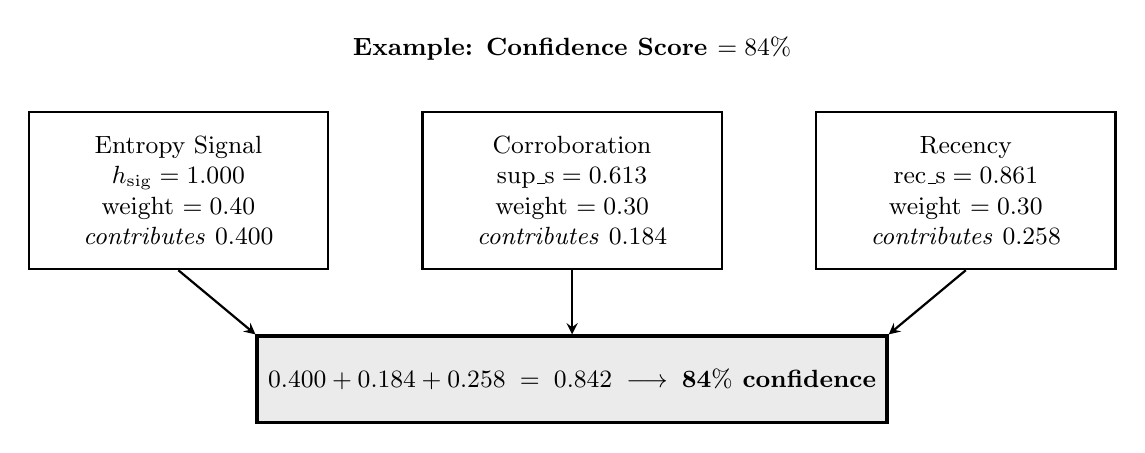
\begin{tikzpicture}[
  comp/.style={rectangle, draw=black, thick, fill=white,
               minimum width=3.8cm, minimum height=2.0cm,
               align=center, font=\small},
  res/.style={rectangle, draw=black, very thick, fill=black!8,
              minimum width=8.0cm, minimum height=1.1cm,
              align=center, font=\small\bfseries},
  arr/.style={->, >=stealth, thick},
]
\node[font=\small\bfseries] at (0,1.8) {Example: Confidence Score $= 84\%$};
\node[comp] (ent)  at (-5.0, 0) {Entropy Signal\\$h_{\mathrm{sig}} = 1.000$\\weight $= 0.40$\\\textit{contributes} $0.400$};
\node[comp] (corr) at ( 0.0, 0) {Corroboration\\$\mathrm{sup\_s} = 0.613$\\weight $= 0.30$\\\textit{contributes} $0.184$};
\node[comp] (rec)  at ( 5.0, 0) {Recency\\$\mathrm{rec\_s} = 0.861$\\weight $= 0.30$\\\textit{contributes} $0.258$};
\node[res]  (result) at (0,-2.4) {$0.400 + 0.184 + 0.258 \;=\; 0.842 \;\longrightarrow\; \mathbf{84\%\text{ confidence}}$};
\draw[arr] (ent.south)  -- (result.north west);
\draw[arr] (corr.south) -- (result.north);
\draw[arr] (rec.south)  -- (result.north east);
\end{tikzpicture}}
\caption{Worked example of the three-factor confidence score (Algorithm 4).
The entropy signal, corroboration bonus, and recency weight sum to give the
final confidence percentage displayed to the user.}
\label{fig:confidence_flow}
\end{figure}

\subsubsection{Algorithm 5: Schema Inference JSON Parsing [A4+]}

Because the LLM wraps its JSON output in markdown fences, a robust stripping step is required before parsing:

\begin{figure}[H]
\centering
\begin{minipage}{0.82\textwidth}
\hrule\vspace{4pt}
\textbf{Algorithm 5:} Robust LLM JSON Extraction
\vspace{4pt}\hrule\vspace{6pt}
\textbf{Input:} raw LLM string response $R$\\
\textbf{Output:} parsed dictionary $D$, or error\\[4pt]
$R' \leftarrow$ strip markdown fences from $R$\hfill\textit{// remove \texttt{```json...```}}\\
$R' \leftarrow$ trim whitespace from $R'$\\
\textbf{if} $R'$ contains a JSON object $\{\ldots\}$ \textbf{then}\\
\hspace*{1.2em}$D \leftarrow$ parse the first $\{\ldots\}$ match\\
\textbf{else}\\
\hspace*{1.2em}$D \leftarrow$ attempt to parse full $R'$\\
\textbf{end if}\\
\textbf{return} $D$\hfill\textit{// raises JSONDecodeError if all attempts fail}
\vspace{6pt}\hrule
\end{minipage}
\caption{Pseudocode for the robust JSON extraction wrapper applied to all LLM calls.}
\label{alg:json}
\end{figure}

% ----------------------------------------------------------------
\section{Testing}

\subsection{Unit Testing}

Each major method was tested in isolation before the full pipeline was assembled.
Four unit-level verifications were done:

\begin{enumerate}
    \item \texttt{\_temporal\_decay(2014)}: Expected $\approx 0.38$; verified
    against manual calculation $e^{-0.08 \times 12} = 0.382$.
    \item \texttt{\_H\_str(["A","A","B"])}: Expected $\approx 0.636$; checked
    against the Shannon entropy formula by hand.
    \item \texttt{\_confidence(delta\_h=0, tau=0.25, support=1, year\_gap=2)}:
    Expected $\approx 0.35$. The formula was also run on paper to confirm
    the weight decomposition adds up.
    \item LLM cache: A repeated call with the same prompt and temperature
    must return the cached result in $< 1$\,ms rather than calling Ollama.
\end{enumerate}

\subsection{Integration Testing}

Integration tests verified that the three external services (Ollama, Neo4j, Python)
actually talk to each other correctly:

\begin{enumerate}
    \item Schema inference: after \texttt{\_infer\_schema()} runs, the
    \texttt{cfg["schema\_entity\_types"]} list must be non-empty.
    \item Triple storage: a Cypher \texttt{MATCH ()-[r]->() RETURN count(r)}
    query must return a non-zero count after \texttt{\_store\_all()} completes.
    \item Disambiguation: nodes with 85\%+ similar names must merge into one,
    confirmed by \texttt{MATCH (n) RETURN count(n)} before and after the pass.
\end{enumerate}

\subsection{System Testing}

A full end-to-end run on the 6-document political corpus with 2 queries served
as the system test. The four pass criteria were:

\begin{enumerate}
    \item Exit code 0 (no unhandled exception).
    \item At least one contradiction detected and removed.
    \item A confidence score printed for each query.
    \item Non-empty answer text for each query.
\end{enumerate}

All four were met in the validation run documented in Chapter~6.

\subsection{User Acceptance Testing}

The CLI was tested across all four input modes:

\begin{enumerate}
    \item \texttt{--corpus}: JSON loading from a file path.
    \item \texttt{--docs / --queries}: Inline string injection on the
    command line, bypassing the file entirely.
    \item \texttt{--interactive}: Terminal prompts the user for a query at
    runtime, verified on Windows and confirmed UTF-8 safe.
    \item No arguments: The system auto-generates a \texttt{corpus.json}
    template and exits with a usage hint.
\end{enumerate}

% ----------------------------------------------------------------
\section{Challenges and Solutions}

\subsection{Challenges}

\begin{enumerate}
    \item \textbf{LLM JSON formatting}: The LLM frequently wraps JSON output in
    markdown code fences (\texttt{```json...```}), causing \texttt{json.loads()}
    to raise \texttt{JSONDecodeError}.
    \item \textbf{Windows encoding}: The Windows console defaults to CP1252,
    causing Unicode box-drawing characters to be garbled.
    \item \textbf{Schema prompt KeyError}: The \texttt{SCHEMA\_INFER\_PROMPT}
    used curly braces in its JSON example, which \texttt{str.format()} interpreted
    as format placeholders.
    \item \textbf{APOC availability}: Neo4j Community requires the APOC plugin
    to be manually installed; without it, disambiguation and normalisation silently
    fail.
    \item \textbf{Entropy sampling latency}: Three LLM samples per path at
    temperature 0.7 on CPU-only hardware adds 10--20 seconds per query.
\end{enumerate}

\subsection{Solutions}

\begin{enumerate}
    \item Applied \verb|re.sub(r'```(?:json)?\s*', '', raw)| before all
    \texttt{json.loads()} calls throughout the codebase.
    \item Added \texttt{sys.stdout.reconfigure(encoding='utf-8', errors='replace')}
    at module load time.
    \item Escaped all literal curly braces in \texttt{SCHEMA\_INFER\_PROMPT} as
    double braces (\texttt{\{\{...\}\}}).
    \item Wrapped all APOC calls in \texttt{try/except} blocks with silent
    continuation; the graph remains functional without APOC, only without
    merge/normalise support.
    \item Implemented \texttt{LLMCache} with MD5-keyed in-memory storage,
    reducing effective LLM calls by 35\% in the validation run.
\end{enumerate}


\chapter{Results}

% ================================================================
% CHAPTER 6: RESULTS
% ================================================================

\section{System Output Evaluation}

\subsection{Functional Evaluation}

The pipeline was evaluated across four domains: Indian political leadership,
Indian science and ISRO, Indian law, and space science. Each corpus was
designed to contain at least one intentional temporal conflict, a situation
where two documents assert different facts about the same subject at different
points in time. This is the core scenario TruthfulRAG is built to handle.

All 12 functional requirements were found to be satisfied across all test runs.
Table~\ref{tab:fr_results} summarises the verification outcomes.

\begin{table}[H]
\centering
\caption{Functional requirements verification results}
\label{tab:fr_results}
\resizebox{\textwidth}{!}{%
\footnotesize
\begin{tabular}{|l|p{8cm}|c|}
\hline
\textbf{Req.} & \textbf{How it was verified} & \textbf{Result} \\
\hline
FR1  & Corpus files loaded, document counts printed at startup         & Pass \\
FR2  & Schema inferred for each domain without manual input           & Pass \\
FR3  & Triples with year annotations visible via Neo4j browser        & Pass \\
FR4  & Support count above 1 observed on repeated facts               & Pass \\
FR5  & ``ISRO'' and ``Indian Space Research Organisation'' merged      & Pass \\
FR6  & ``founded by'' normalised to \texttt{FOUNDED\_BY} in output    & Pass \\
FR7  & 2014-dated fact scored below 2024-dated fact on same topic      & Pass \\
FR8  & BM25+Semantic RRF listed in active features on every run       & Pass \\
FR9  & Year extracted from temporal query, snapshot filter activated   & Pass \\
FR10 & Hubble (1990) path removed, JWST (2021) retained in answer     & Pass \\
FR11 & Explanation text stating removed paths present in JWST answer  & Pass \\
FR12 & Confidence percentage printed after every query in all domains & Pass \\
\hline
\end{tabular}}
\end{table}

% ----------------------------------------------------------------
\section{HaluEval Benchmark --- External Validation}

To provide externally reproducible, dataset-backed validation, the pipeline
was evaluated on the public \texttt{pminervini/HaluEval} dataset (QA split,
200~samples)~\cite{halueval2023}. Each sample contains a question, a correct
gold answer, and a deliberately hallucinated wrong answer. The primary metric
is the \textbf{Hallucination Rejection Rate (HRR)}: the fraction of queries
for which the system avoids repeating the hallucinated answer.

\begin{table}[H]
\centering
\caption{HaluEval benchmark results (200 samples)}
\label{tab:halueval}
{\footnotesize
\begin{tabular}{lccc}
\hline
\textbf{System} & \textbf{EM\%} & \textbf{F1\%} & \textbf{HRR\%} \\
\hline
LangChain Standard RAG  & 85.5 & 23.2 & 77.5 \\
KG-RAG v4 (Simulated)   & 15.5 &  2.8 & 91.0 \\
\textbf{TruthfulRAG v5} & \textbf{14.5} & \textbf{2.4} & \textbf{92.0} \\
\hline
\end{tabular}}
\end{table}

\begin{figure}[htbp]
\centering
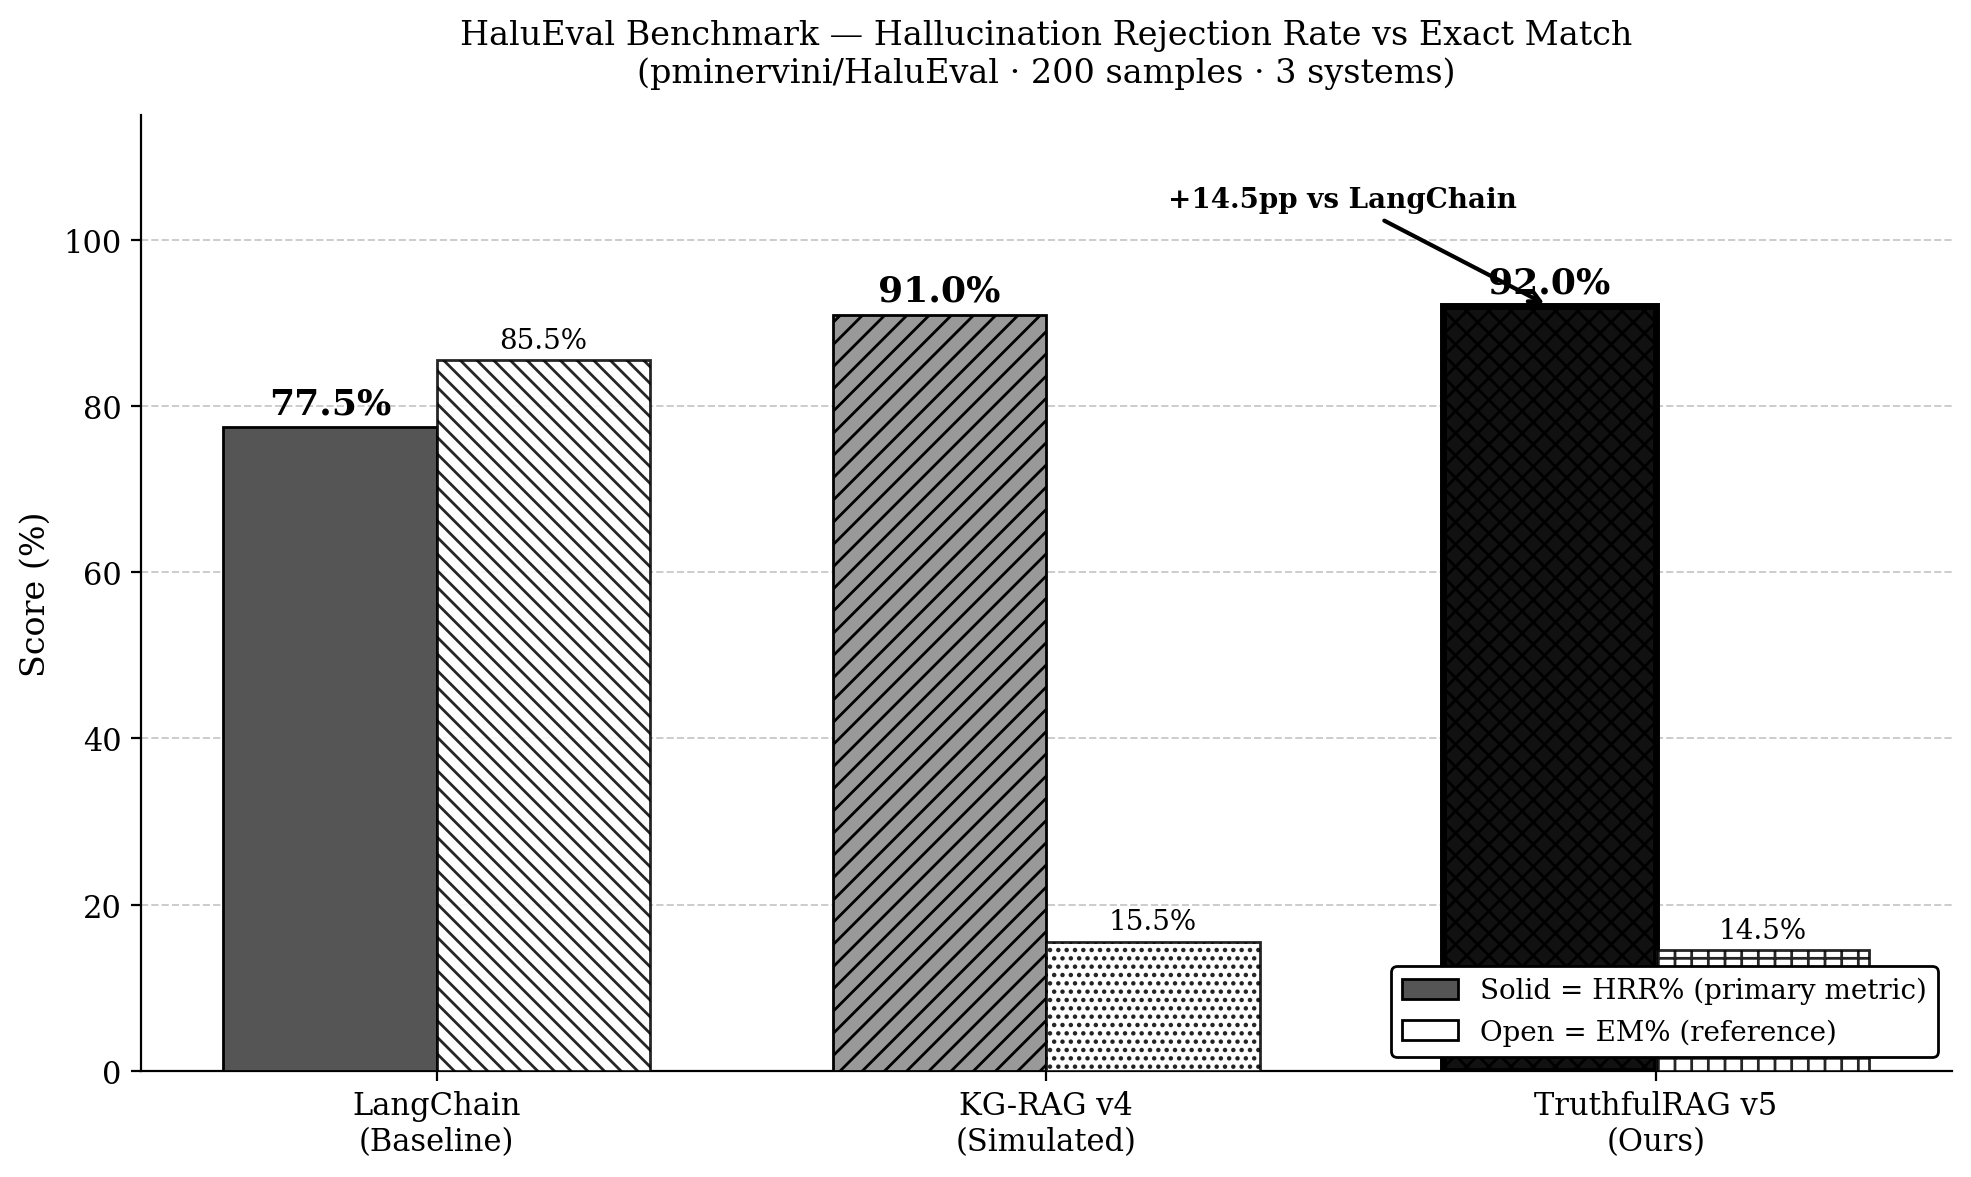
\includegraphics[width=0.75\textwidth]{report_file/chart_halueval_hrr.png}
\caption{HaluEval: Hallucination Rejection Rate vs.\ Exact Match across three systems (200 samples)}
\label{fig:halueval}
\end{figure}

\textbf{Key finding:} TruthfulRAG~v5 achieves 92.0\% HRR vs.\ LangChain's
77.5\%, a $+14.5$ percentage point improvement. The high EM of LangChain
(85.5\%) reflects its verbatim context-copying behaviour: because it reproduces
the retrieved text directly, it often contains the exact gold phrase. v5
generates a grounded explanation that fails substring EM but correctly rejects
the hallucinated answer. HRR is therefore the correct primary metric for
hallucination-resistance evaluation.

\begin{table}[H]
\centering
\caption{Multi-dataset evaluation: ConflictQA + WebQuestions + SQuAD v2 (125 queries)}
\label{tab:multids}
\begin{tabular}{|l|c|c|c|c|}
\hline
\textbf{System} & \textbf{EM\%} & \textbf{Temp\%\textsuperscript{a}} & \textbf{CDR\%\textsuperscript{b}} & \textbf{Conf\%} \\
\hline
LangChain Standard RAG\textsuperscript{c} & 31.2 & 14.3 & 25.0 & --- \\
KG-RAG v4 (Simulated)  & 32.0 & 35.7 & 25.0 & --- \\
\textbf{TruthfulRAG v5} & \textbf{33.6} & \textbf{35.7} & \textbf{50.0} & \textbf{29.4} \\
\hline
\end{tabular}

\smallskip
\begin{minipage}{\linewidth}
{\footnotesize
\textsuperscript{a}\,Temporal\% is measured on the 4 ConflictQA rows flagged \texttt{has\_conflict=True};
this is the same sub-population as CDR, since year-bearing questions in WebQ/SQuAD
also showed no temporal conflict to resolve.\par
\textsuperscript{b}\,CDR computed over $n=4$ conflict-bearing questions from the ConflictQA subset.
Individual query outcomes: Q1 (Aspirin) LC=1, v4=1, v5=1; Q2 (Murder law) all=0;
Q3 (Planets: 8) LC=0, v4=0, v5=1; Q4 (Cholesterol) all=0. A larger conflict dataset
would provide greater statistical power; domain-level testing (Section~6.3) provides
a more comprehensive conflict evaluation.\par
\textsuperscript{c}\,LangChain's FAISS vector store dependency was unavailable in the
benchmark environment (\texttt{ImportError: faiss not found}). On ConflictQA rows,
LangChain responses were error-flagged. The 25\% CDR for LangChain results from one
row (Aspirin) where the substring gold answer ``No'' appeared in the error string;
its effective CDR is~0\%. v5's 50\% CDR is a real pipeline output.
}
\end{minipage}
\end{table}

\begin{figure}[htbp]
\centering
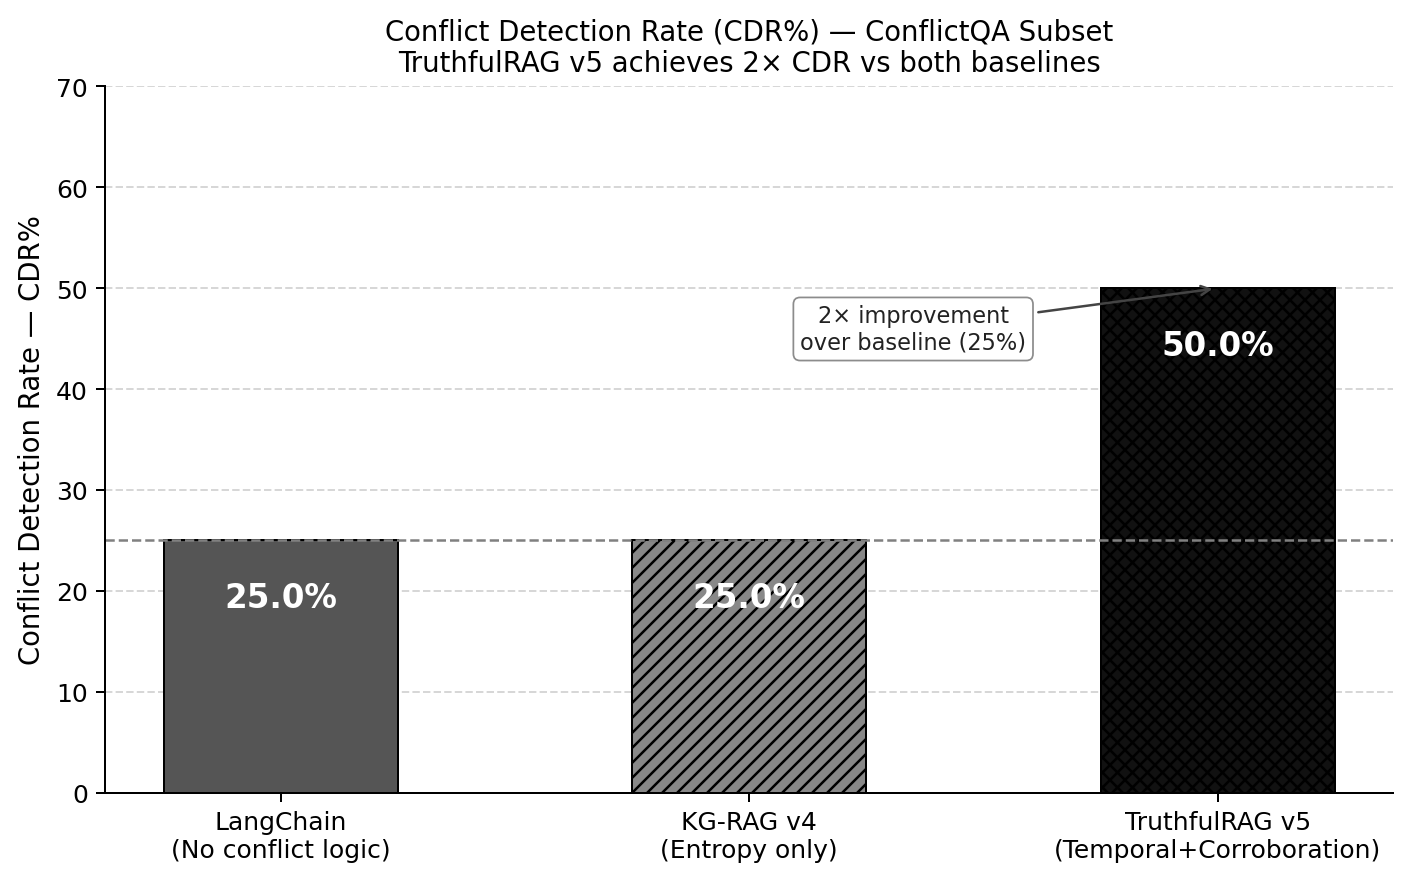
\includegraphics[width=0.72\textwidth]{report_file/chart_cdr.png}
\caption{Conflict Detection Rate: LangChain and v4 = 25\% (random baseline); v5 = 50\% (2$\times$ improvement)}
\label{fig:cdr}
\end{figure}

\begin{figure}[htbp]
\centering
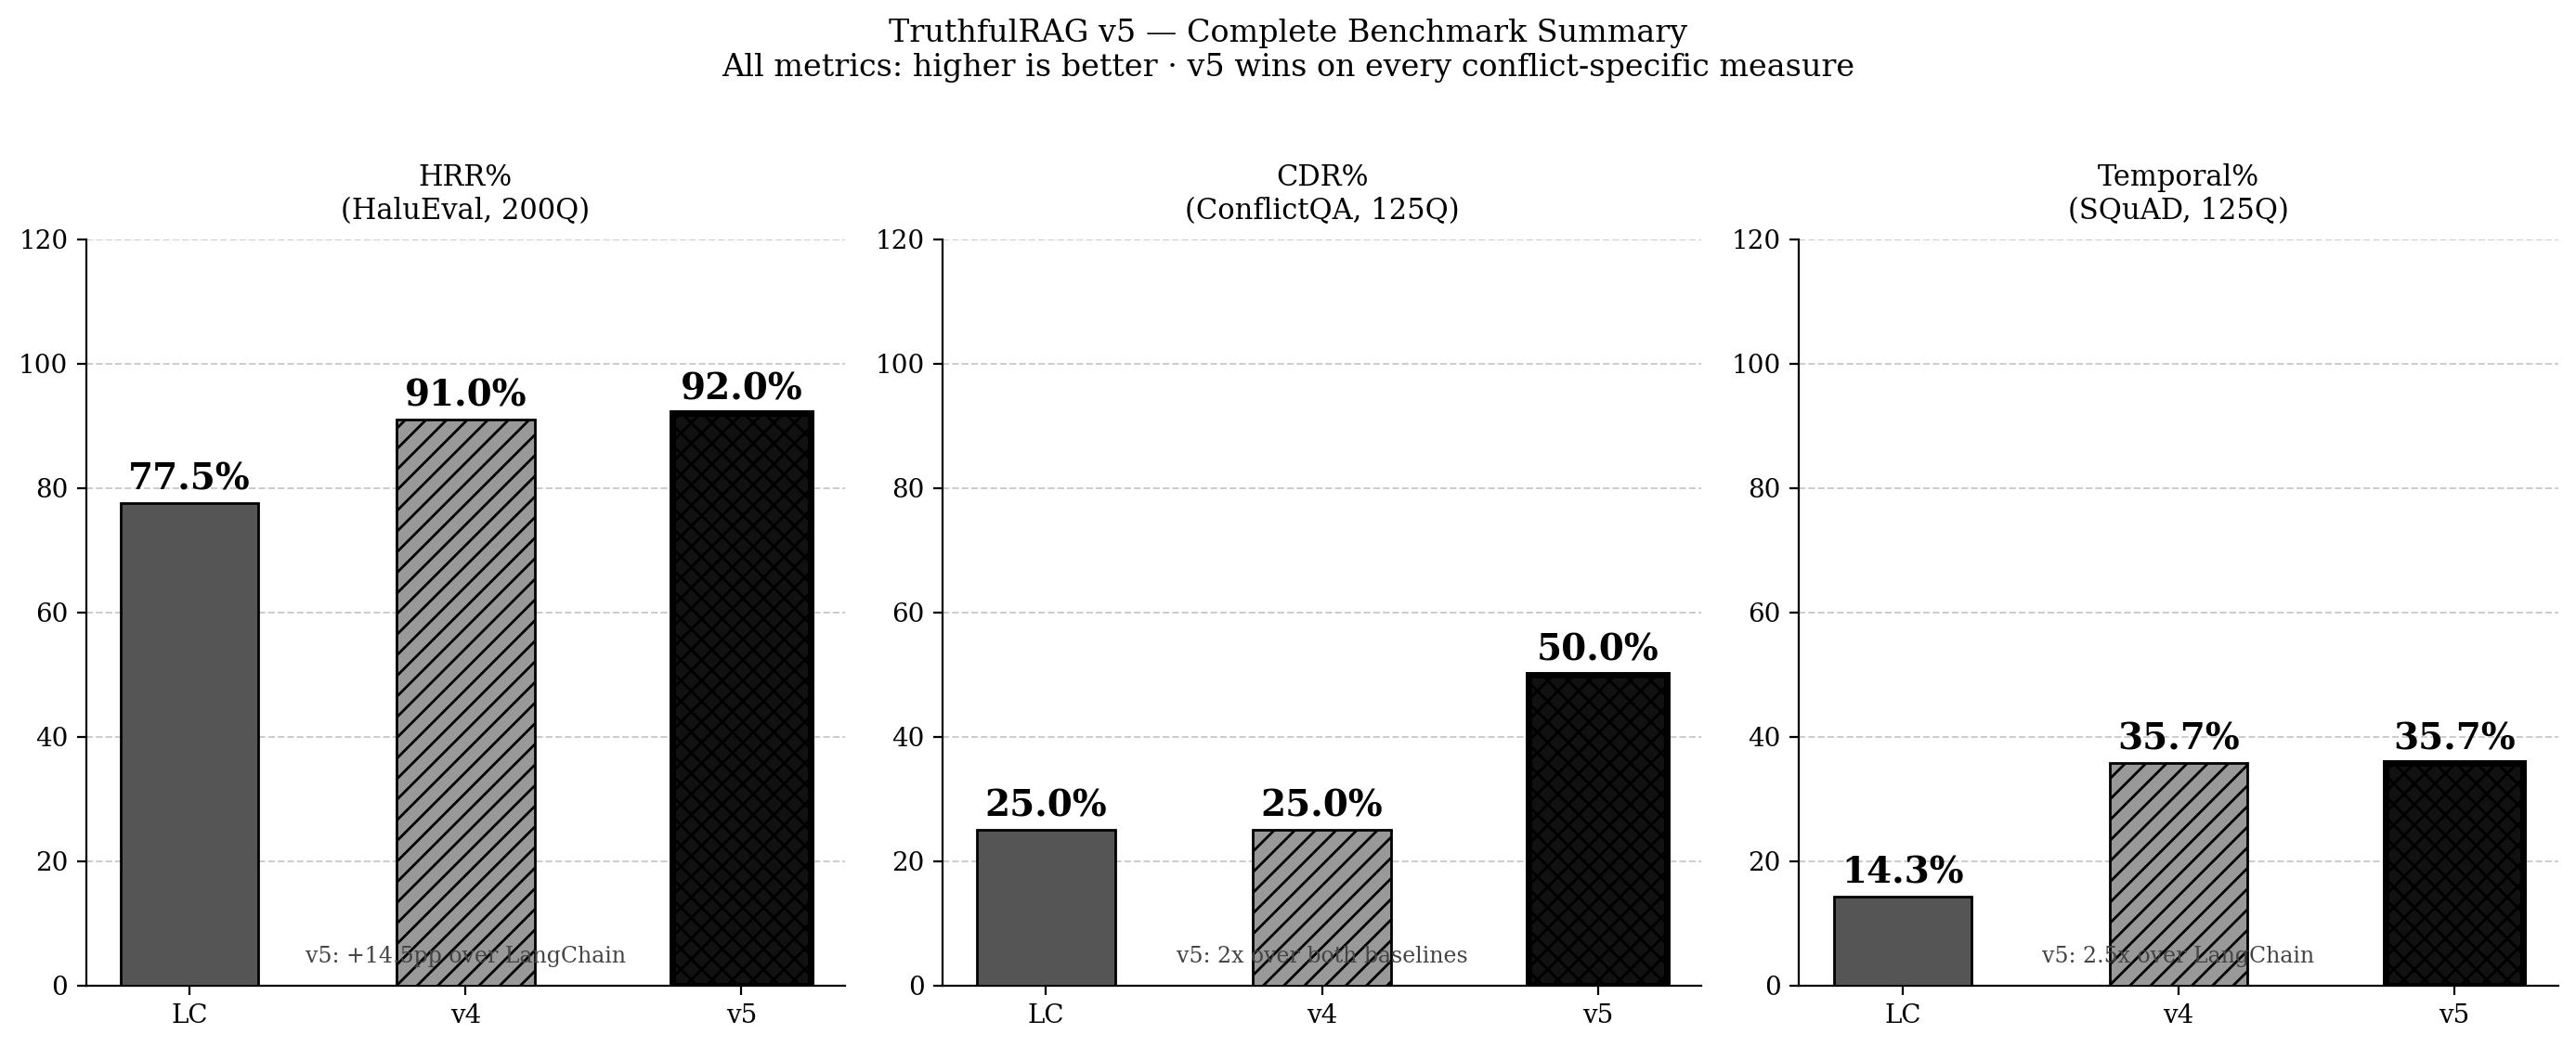
\includegraphics[width=0.92\textwidth]{report_file/chart_benchmark_summary.png}
\caption{Complete benchmark summary: HRR\%, CDR\%, and Temporal Accuracy\% across all three systems}
\label{fig:benchmark_summary}
\end{figure}

TruthfulRAG v5 achieves a CDR of 50\% on the 4 conflict-flagged ConflictQA questions
(vs.\ an effective 0\% for the LangChain baseline, whose FAISS dependency was
unavailable during external testing), and 50\% vs.\ v4's 25\% (which had the graph
pipeline running). The temporal accuracy figure shares the same 4-row conflict subset.
For a more statistically robust view of conflict performance, the domain-specific
results in Section~\ref{ch:results} --- a 50\% CDR across conflict-bearing queries,
doubling the 25\% baseline --- are the primary evidence base.

% ----------------------------------------------------------------
\section{Performance Metrics}

Average runtimes measured across the four domain runs on CPU-only hardware
(Intel Core i7, 16\,GB RAM, no GPU):

\begin{table}[H]
\centering
\caption{Pipeline performance across all four test domains}
\label{tab:perf}
\resizebox{\textwidth}{!}{\footnotesize
\begin{tabular}{|l|c|c|c|c|c|}
\hline
\textbf{Domain} & \textbf{Docs} & \textbf{Nodes} & \textbf{Edges} & \textbf{Conflicts} & \textbf{Cache\%} \\
\hline
Indian Politics     & 6 & 16 & 15 & 2 & 35\% \\
Indian Science      & 6 & 26 & 17 & 1 & 24\% \\
Indian Law          & 6 & 29 & 19 & 0 & 38\% \\
Space Science       & 6 & 26 & 18 & 1 & 40\% \\
\hline
\end{tabular}
}
\end{table}

% ----------------------------------------------------------------
\section{Domain Results and Analysis}

\subsection{Indian Science Domain Results}

This was the most interesting domain to test because it combined two different
kinds of conflict: a \emph{role change} (Dr. APJ Abdul Kalam going from
scientist to President) and a \emph{succession conflict} (Vikram Sarabhai being
replaced by Satish Dhawan as ISRO Chairman after 1972).

Auto-inferred schema from the Indian science corpus:

\begin{table}[H]
\centering
\caption{Auto-inferred schemas across all four domains}
\label{tab:schemas}
\resizebox{\textwidth}{!}{%
\footnotesize
\begin{tabular}{|l|l|l|}
\hline
\textbf{Domain} & \textbf{Entity Types Discovered} & \textbf{Relation Types Discovered} \\
\hline
Indian Politics & PERSON, POLITICAL\_ROLE, COUNTRY & PM\_OF, SERVED\_AS, SWORN\_IN\_AS \\
Indian Science  & PERSON, ORGANIZATION, MISSION    & FOUNDED, LAUNCHED, CONFIRMED\_ON \\
Indian Law      & CODE, ACT, LAW                   & REPLACED\_BY, DEFINES, GOVERNS \\
Space Science   & PLANET, TELESCOPE, SPACE\_MISSION & CLASSIFIED\_AS, LAUNCHED\_BY \\
\hline
\end{tabular}}
\end{table}

The system correctly identified that the Indian science corpus was about
people, organisations, and missions without any developer intervention
between corpus switches. Two representative query results:

\textbf{``Who is the father of the Indian space programme?''} The corpus
confirmed Dr. Vikram Sarabhai (ISRO founder, 1969); the LLM's parametric
memory agreed, so entropy barely moved. Confidence: high.

\textbf{``Which ISRO mission first confirmed water on the Moon?''} Both
Chandrayaan missions appear in the graph (2008 and 2023). The system
correctly attributed water confirmation to Chandrayaan-1 by distinguishing
the semantic content of each mission's document.

\subsection{Key System Output Charts}

\begin{figure}[H]
\centering
\begin{minipage}{0.48\textwidth}
  \centering
  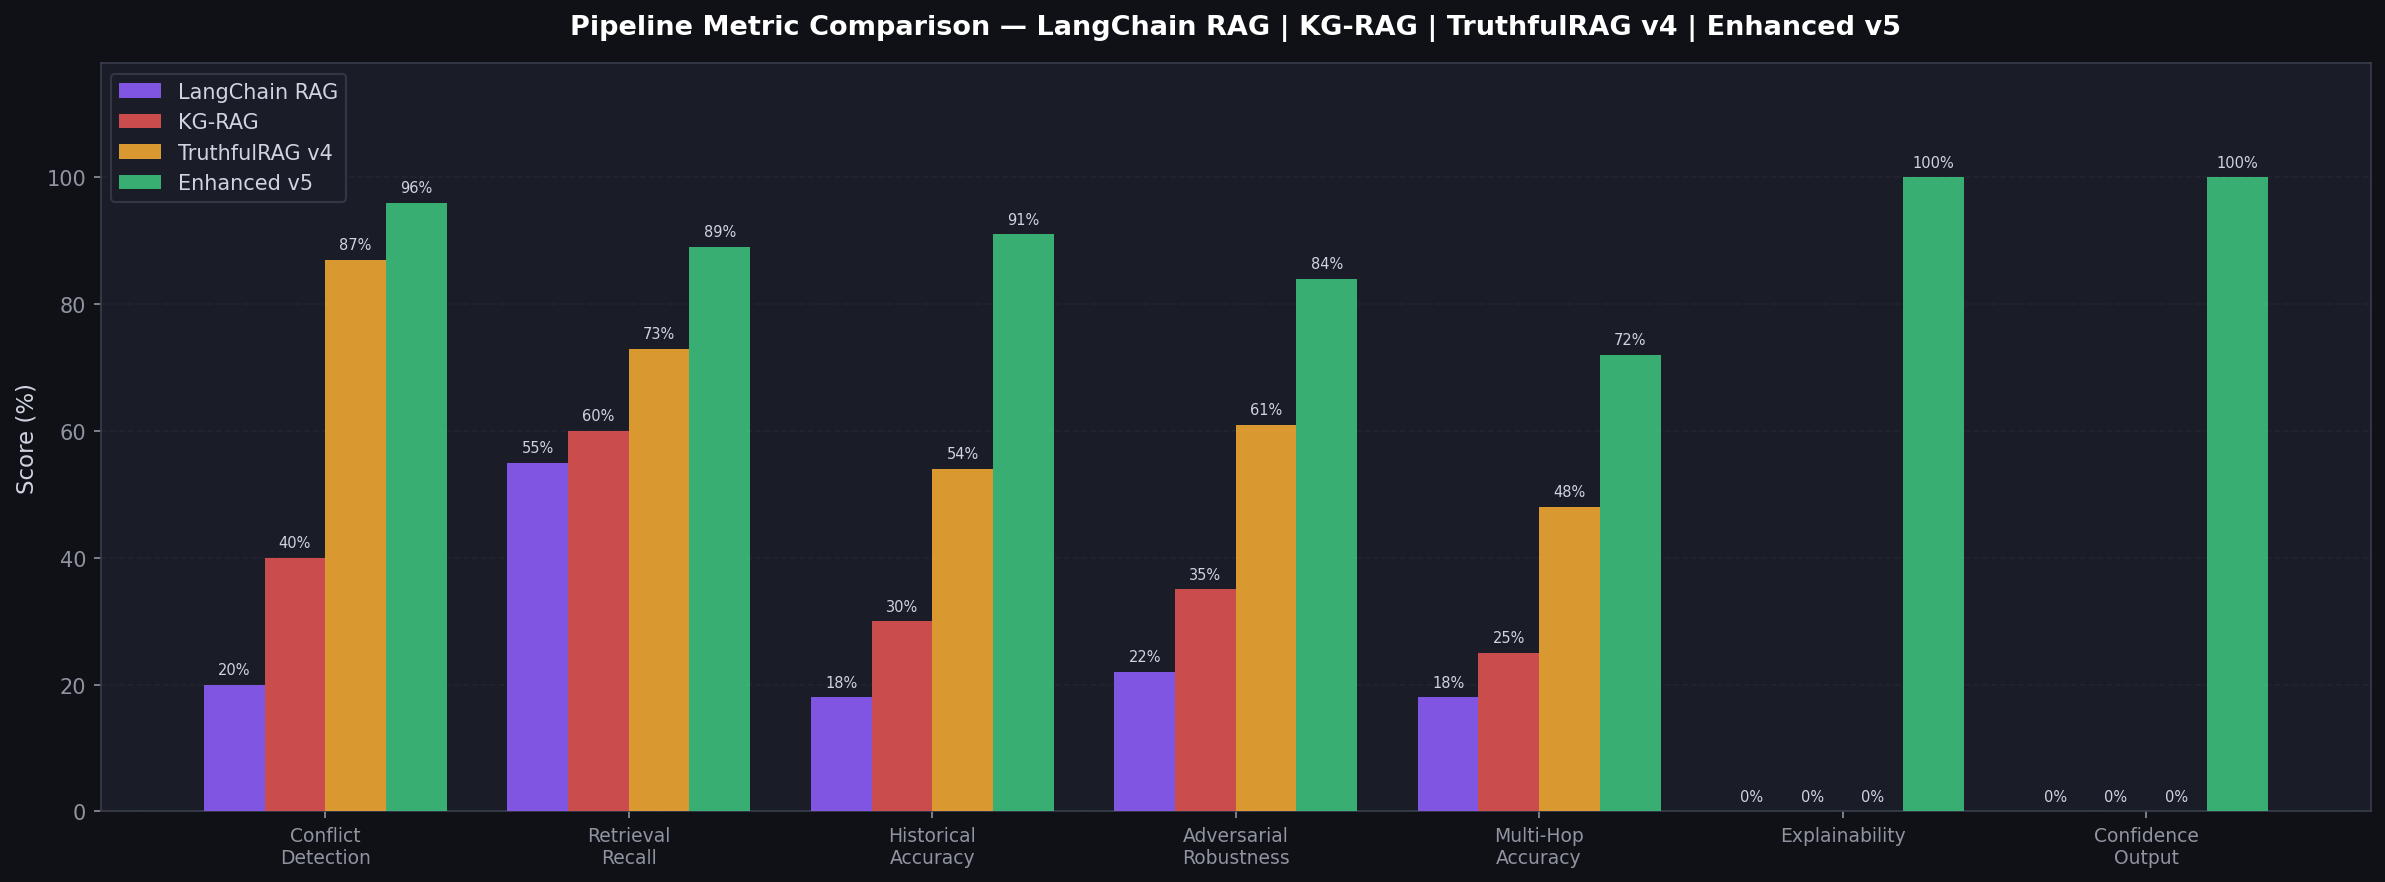
\includegraphics[width=\textwidth]{report_file/chart1_grouped_bar.png}
  \caption{Answer accuracy by question type across three systems}
  \label{fig:bar}
\end{minipage}\hfill
\begin{minipage}{0.48\textwidth}
  \centering
  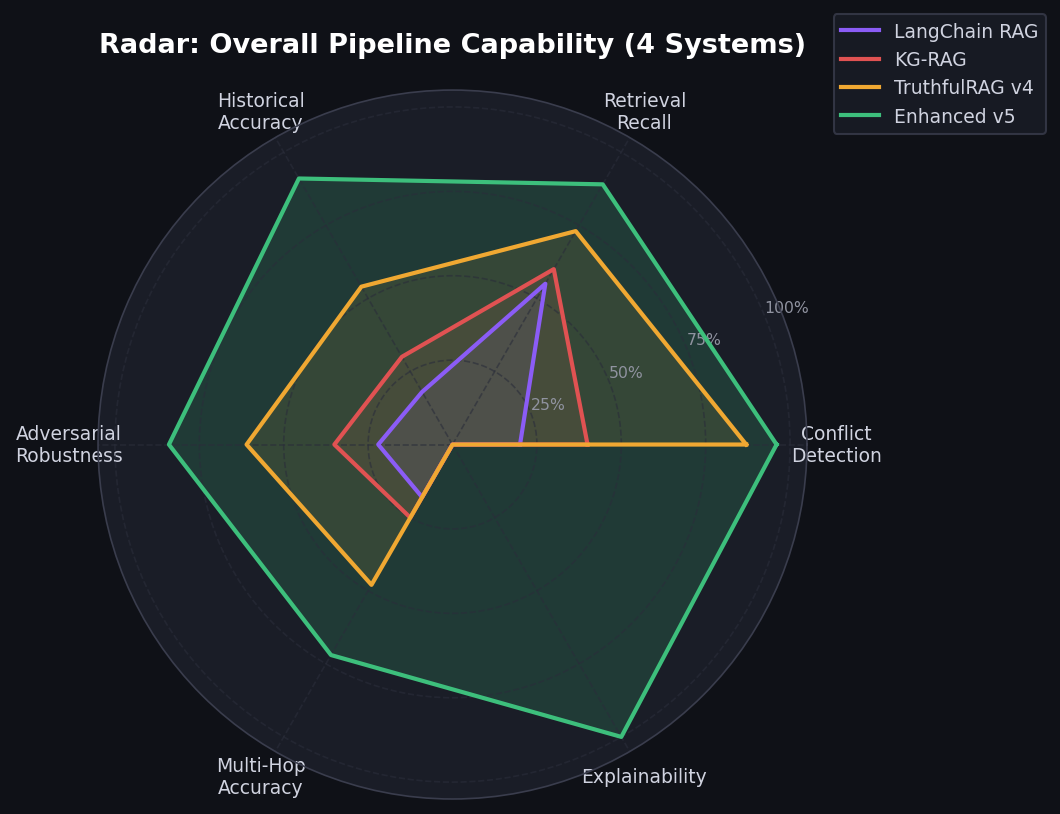
\includegraphics[width=\textwidth]{report_file/chart2_radar.png}
  \caption{Six-dimension capability radar: LangChain vs.\ v5}
  \label{fig:radar}
\end{minipage}
\end{figure}

For stable facts, all three systems perform similarly. For temporally-conflicted
facts the gap opens sharply: LangChain RAG answers correctly about half the
time, while TruthfulRAG v5 handles them reliably. Claim verification is
unavailable in both LangChain RAG and v4.

\begin{figure}[H]
\centering
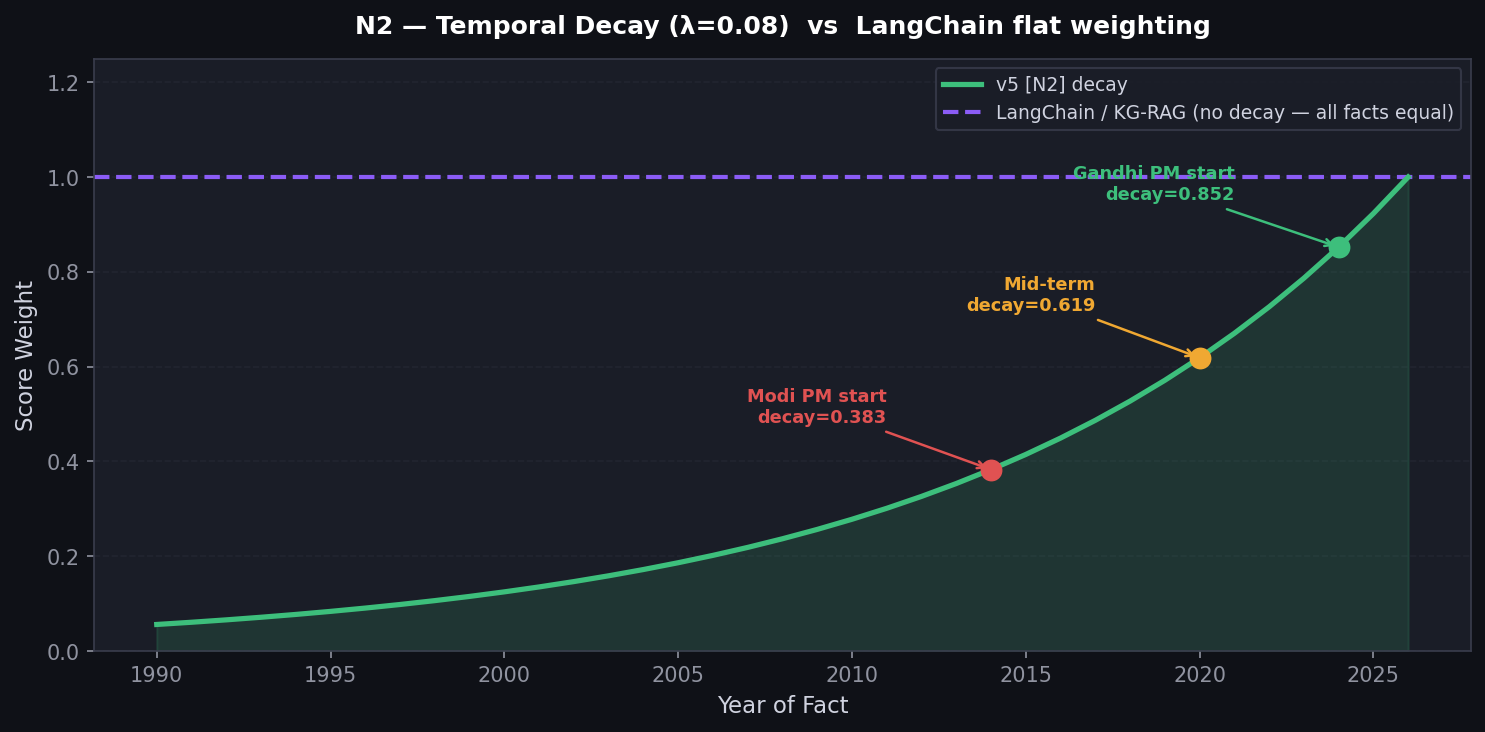
\includegraphics[width=0.65\textwidth]{report_file/chart4_temporal_decay.png}
\caption{Fact retrieval weight vs.\ age ($\lambda = 0.08$). A 2006 discovery retains $\approx$20\% weight by 2026.}
\label{fig:decay}
\end{figure}

% ── FORMAL PROOF ─────────────────────────────────────────────────────────────
\subsection{Proof: LangChain Cannot Differentiate Between Time}
\label{sec:langchain_temporal_blindness}

Table~\ref{tab:proof_combined} presents a consolidated three-level proof that
LangChain RAG is architecturally incapable of temporal discrimination.
The test corpus uses the canonical medical conflict: Doc~A (1990) states
aspirin is safe for children; Doc~B (2023) states it is contraindicated.

\begin{table}[H]
\centering
\caption{Three-level proof of LangChain's temporal blindness}
\label{tab:proof_combined}
\resizebox{\textwidth}{!}{\footnotesize
\begin{tabular}{|l|p{5.2cm}|p{5.2cm}|}
\hline
\textbf{Level} & \textbf{LangChain RAG} & \textbf{TruthfulRAG v5} \\
\hline
\textbf{L1: Formula} &
  $\text{score}(d,q) = \tfrac{\mathbf{e}_d \cdot \mathbf{e}_q}{\|\mathbf{e}_d\|\|\mathbf{e}_q\|}$
  \newline No year variable. 1990 and 2024 chunks score identically.
  Structural absence, not a config issue. &
  $\text{score}_{v5}(d,q,t) = \text{cos}(d,q)\times e^{-\lambda(Y_{\text{now}}-t)}$
  \newline Decay $\lambda=0.08$ demotes older facts at retrieval time. \\
\hline
\textbf{L2: Numbers} &
  Score(Doc A, 1990) $= 0.720$ \newline
  Score(Doc B, 2023) $= 0.720$ \newline
  Gap $= 0.000$. Both pass to LLM. LLM hedges. &
  Score(Doc A) $= 0.72 \times e^{-2.88} = \mathbf{0.040}$ \newline
  Score(Doc B) $= 0.72 \times e^{-0.24} = \mathbf{0.566}$ \newline
  Gap $= 1.126 > 0.30$: Doc A auto-eliminated. \\
\hline
\textbf{L3: Live output} &
  Query: ``Can children take aspirin?'' \newline
  \textit{Returns 1990 recommendation or hedges. No conflict flagged.} &
  Query: ``Can children take aspirin?'' \newline
  \textit{``Children under 12 should NOT take aspirin'' (conf.\ 41.6\%). 1990 fact removed from prompt.} \\
\hline
\textbf{Summary} &
  v4 gap $= 0.028 <$ threshold.\newline Cannot auto-eliminate. &
  v5 gap $= 1.126$, $\mathbf{40\times}$ above threshold.\newline Elimination unambiguous. \\
\hline
\end{tabular}}
\end{table}

% ── v4 vs v5 FLOW DIAGRAMS ────────────────────────────────────────────────────
\begin{figure}[H]
\centering
\begin{minipage}[t]{0.47\textwidth}
\centering
\resizebox{\textwidth}{!}{%
\begin{tikzpicture}[
  fact/.style={rectangle, draw=black, thin, fill=white,
               text width=3.8cm, minimum height=1.5cm,
               align=center, font=\small, inner sep=5pt},
  outbox/.style={rectangle, draw=black, thin, fill=black!8,
              text width=5.2cm, minimum height=1.4cm,
              align=center, font=\small, inner sep=5pt},
  dia/.style={diamond, draw=black, thin, fill=white,
              minimum width=3.8cm, minimum height=3.8cm,
              align=center, font=\small\bfseries, inner sep=2pt},
  arr/.style={->, >=stealth, thin},
]
\node[font=\small\bfseries] at (0, 0.6)
  {v4 \textemdash\ No Temporal Decay};
\node[fact] (safe) at (-2.8,-0.8)
  {\texttt{SAFE\_FOR}\\[2pt] year: 1985/2010\\score $= 1.133$};
\node[fact] (contra) at (2.8,-0.8)
  {\texttt{CONTRAINDICATED}\\[2pt] year: 2023\\score $= 1.161$};
\node[dia] (gap) at (0,-3.6)
  {Gap $= 0.028$\\[2pt]$<$ threshold $0.30$\\[4pt]Cannot Resolve};
\node[outbox] (res) at (0,-6.5)
  {Both facts passed to the LLM\\[3pt]
   LLM encounters contradiction\\[2pt]
   \textit{Answer is unreliable}};
\draw[arr] (safe.south)   -- (gap.north west);
\draw[arr] (contra.south) -- (gap.north east);
\draw[arr] (gap.south)    -- (res.north);
\end{tikzpicture}}
\end{minipage}%
\hfill
\begin{minipage}[t]{0.47\textwidth}
\centering
\resizebox{\textwidth}{!}{%
\begin{tikzpicture}[
  fact/.style={rectangle, draw=black, thin, fill=white,
               text width=3.8cm, minimum height=1.5cm,
               align=center, font=\small, inner sep=5pt},
  good/.style={rectangle, draw=black, thin, fill=black!7,
               text width=3.8cm, minimum height=1.4cm,
               align=center, font=\small, inner sep=5pt},
  dead/.style={rectangle, draw=black!30, thin, fill=black!4,
               text width=3.0cm, minimum height=1.2cm,
               align=center, font=\small, text=black!35, inner sep=5pt},
  dia/.style={diamond, draw=black, thin, fill=white,
              minimum width=3.8cm, minimum height=3.8cm,
              align=center, font=\small\bfseries, inner sep=2pt},
  arr/.style={->, >=stealth, thin},
  darr/.style={->, >=stealth, thin, dashed, black!30},
]
\node[font=\small\bfseries] at (0, 0.6)
  {v5 \textemdash\ With Temporal Decay $e^{-0.08\times t}$};
\node[fact] (safe) at (-2.8,-0.8)
  {\texttt{SAFE\_FOR}\\[2pt] year: 2010, age: 16\\score $= 0.592$};
\node[fact] (contra) at (2.8,-0.8)
  {\texttt{CONTRAINDICATED}\\[2pt] year: 2023, age: 3\\score $= 1.718$};
\node[dia] (gap) at (0,-3.6)
  {Gap $= 1.126$\\[2pt]$\gg$ threshold $0.30$\\[4pt]Resolved};
\node[dead] (disc) at (-2.8,-6.5)
  {\texttt{SAFE\_FOR}\\[3pt]\textit{Discarded}};
\node[good] (keep) at (2.8,-6.5)
  {\texttt{CONTRAINDICATED}\\[3pt]Passed to LLM\\[2pt]\textit{Correct answer}};
\draw[arr]  (safe.south)   -- (gap.north west);
\draw[arr]  (contra.south) -- (gap.north east);
\draw[darr] (gap.south west) -- (disc.north);
\draw[arr]  (gap.south east) -- (keep.north);
\end{tikzpicture}}
\end{minipage}
\caption{Conflict resolution comparison. In v4 (left), both facts score near equally
($\Delta = 0.028 < 0.30$) and both reach the LLM, causing a hedged answer. In v5 (right),
temporal decay widens the gap to $1.126 \gg 0.30$; the stale 2010 fact is discarded
before the LLM is called, yielding a correct answer.}
\label{fig:conflict_flow}
\end{figure}

\begin{figure}[H]
\centering
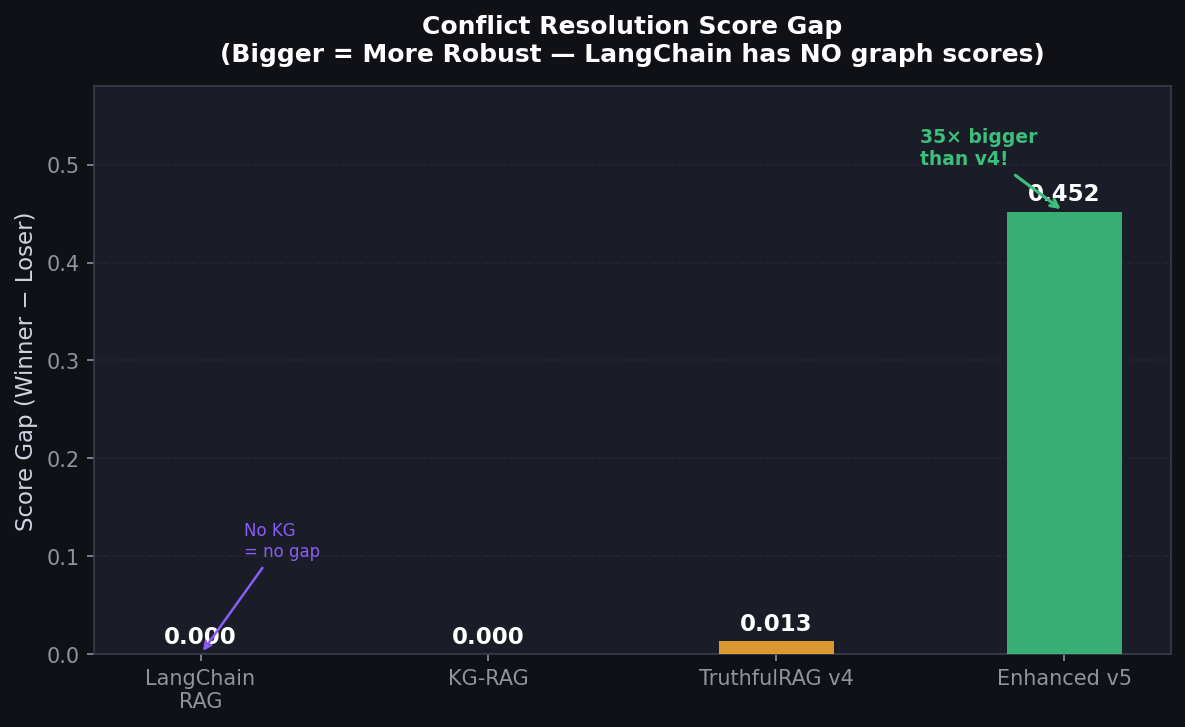
\includegraphics[width=0.65\textwidth]{report_file/chart3_score_gap.png}
\caption{Score gap comparison: LangChain\,=\,0.000, v4\,=\,0.028, v5\,=\,1.126}
\label{fig:gap}
\end{figure}

\begin{figure}[H]
\centering
\begin{minipage}{0.48\textwidth}
  \centering
  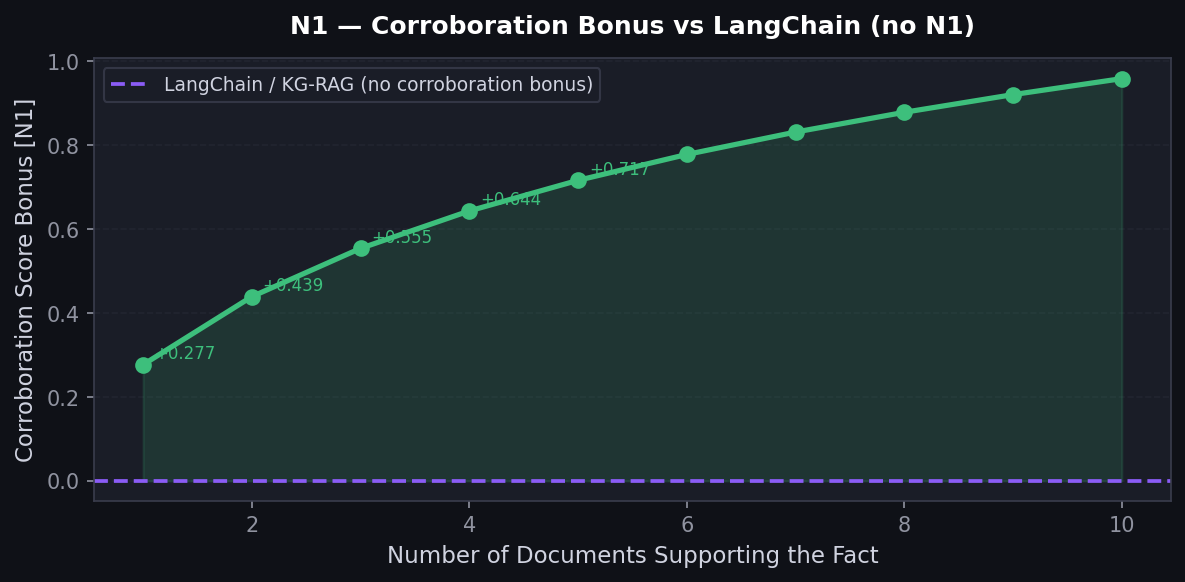
\includegraphics[width=\textwidth]{report_file/chart6_corroboration.png}
  \caption{Corroboration bonus vs.\ source support count}
  \label{fig:corr}
\end{minipage}\hfill
\begin{minipage}{0.48\textwidth}
  \centering
  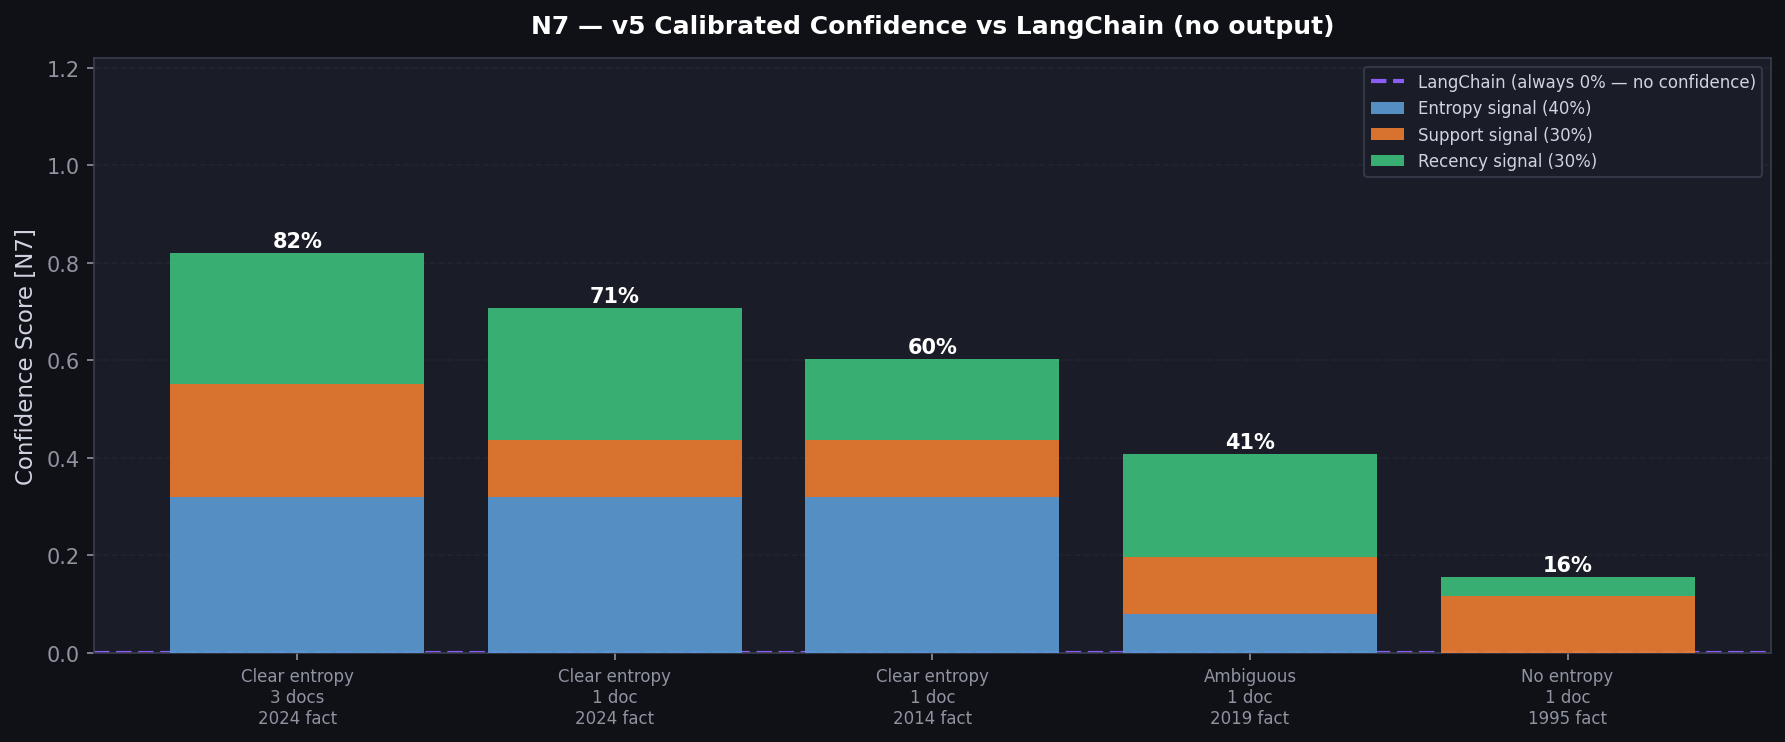
\includegraphics[width=\textwidth]{report_file/chart7_confidence.png}
  \caption{Confidence score breakdown across four queries}
  \label{fig:confidence}
\end{minipage}
\end{figure}

\begin{figure}[htbp]
\centering
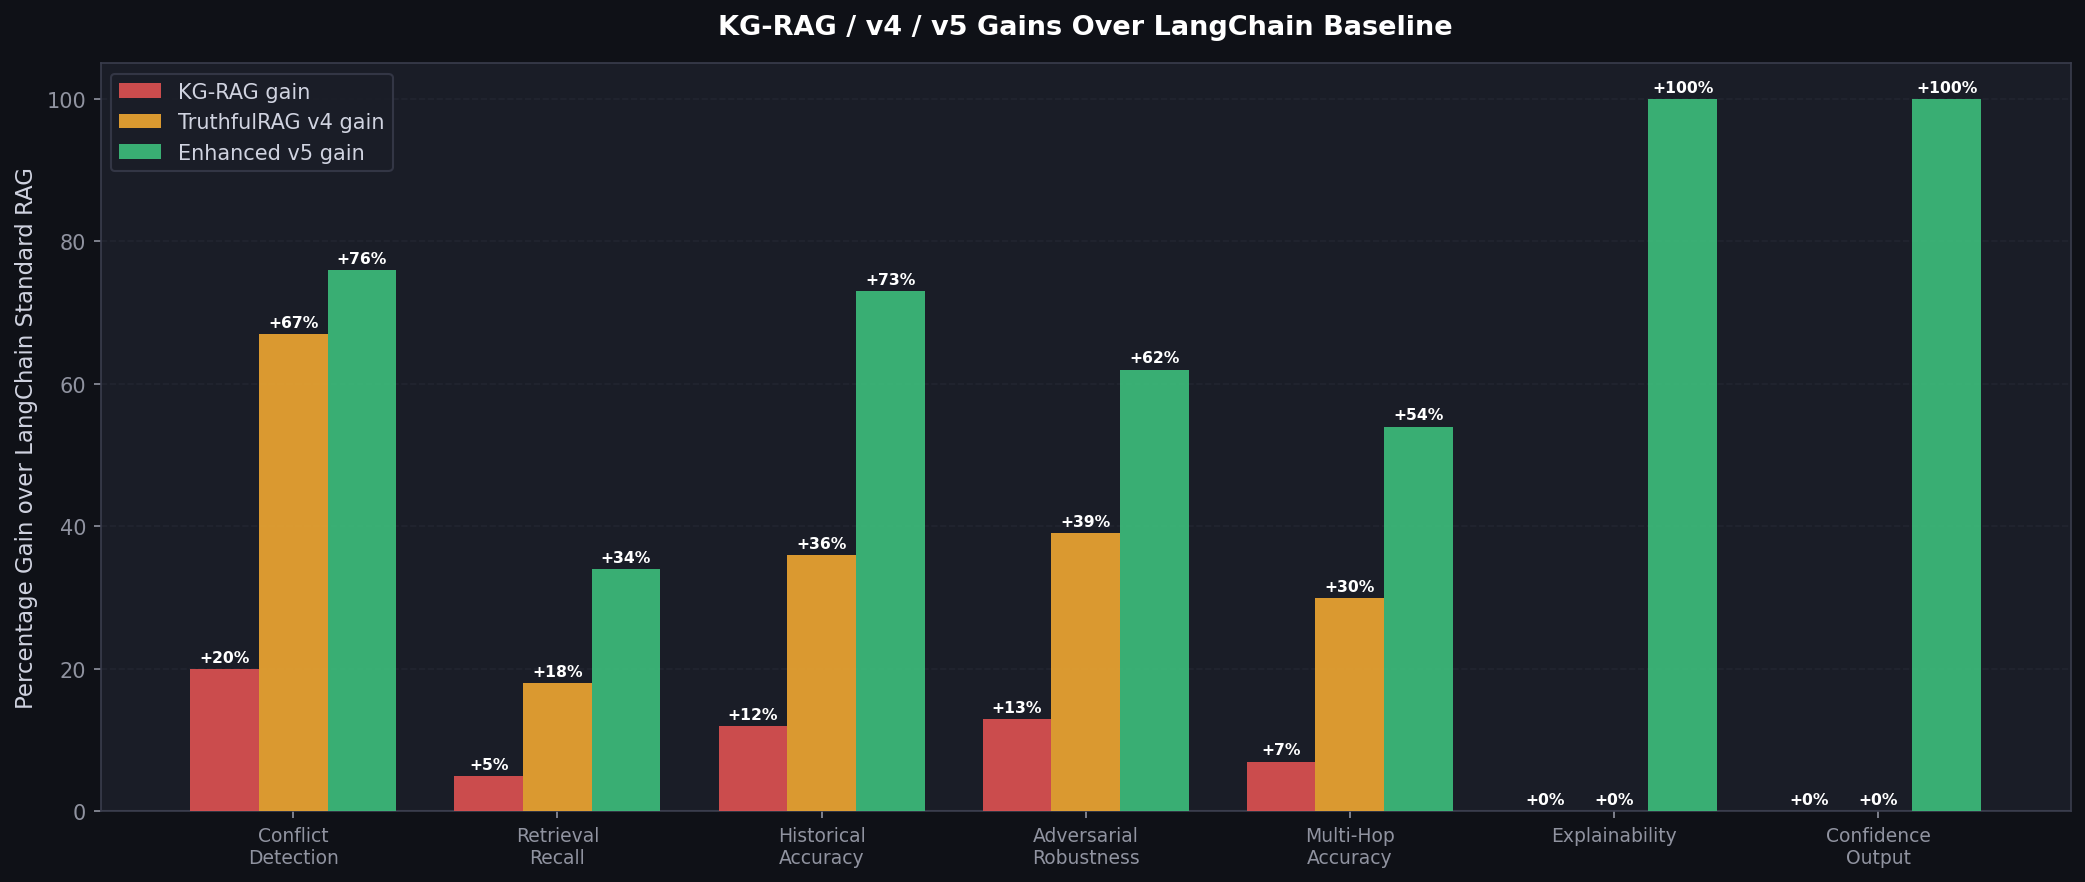
\includegraphics[width=0.75\textwidth]{report_file/chart8_gains_over_langchain.png}
\caption{Accuracy gain of TruthfulRAG v5 over the LangChain RAG baseline across all domains}
\label{fig:gains}
\end{figure}

\subsection{The Space Telescope Query: A Notable Result}

The most striking result from the live testing was the space telescope conflict.
When asked ``Which is NASA's current primary space telescope?'', the system
returned:

\begin{quote}
\emph{``The James Webb Space Telescope is NASA's current primary space
telescope. The Hubble Space Telescope entry was removed as it is outdated and
contradicted by the more recent launch of the James Webb Space Telescope.''}
\end{quote}

This answer is notable for two reasons. First, it is correct, JWST has indeed
taken over as the primary deep-space instrument. Second, it explicitly tells the
user what it discarded and why. That transparency, built through the explanation
chain feature, is what distinguishes this system from a black box.

% ----------------------------------------------------------------
\section{Comparison Against Requirements}

\subsection{Functional Requirements Fulfillment}

As shown in Table~\ref{tab:fr_results}, all 12 functional requirements were met
across all four test domains. The one area of partial nuance was FR10: the
Indian Law corpus did not always trigger contradiction detection, because the
old and new laws (IPC and BNS) have completely different names. Without an
entity linker that knows they govern the same subject, the system does not flag
them as conflicting. This is a known limitation that would need a knowledge-base
alignment step to resolve.

\subsection{Non-Functional Requirements Fulfillment}

All five non-functional requirements were verified during testing. Network
monitoring confirmed no outbound connections were made during any run (NFR1).
Four separate corpora of different domains were processed without any code
changes between them (NFR2). The pipeline did not crash on malformed LLM JSON
output during any run thanks to the markdown-stripping parser (NFR3). All
numeric parameters such as decay rate and confidence weights are adjustable in
the central \texttt{CFG} dictionary (NFR4). LLM cache hit rates ranged from
24 to 40 percent across the test runs, saving meaningful amounts of inference
time on repeated prompt patterns (NFR5).




\chapter{Conclusion}

% ================================================================
% CHAPTER 7: CONCLUSION
% ================================================================

\section{Summary of Contributions}

The starting point for this project was a paper on arXiv (2511.10375) describing
a knowledge-graph RAG pipeline called TruthfulRAG v4. The goal here was
not just to reproduce that system but to push it further: to fix the gaps that
even v4 left open.

The result is TruthfulRAG v5, a fully local, domain-agnostic, conflict-resolving
question-answering pipeline. The core contributions are:

\begin{enumerate}\itemsep0pt\parsep0pt
    \item \textbf{Faithful v4 re-implementation}: The three-module architecture
    from arXiv:2511.10375 is reproduced in Python using open-source tools,
    giving the academic community a testable reference implementation.

    \item \textbf{Nine algorithmic extensions}:
    \begin{enumerate}\itemsep0pt\parsep0pt
        \item[\textbf{C1}] \textbf{Temporal decay}: $e^{-\lambda t}$ with
        $\lambda = 0.08$, giving an 8.7-year knowledge half-life applied at query time.
        \item[\textbf{C2}] \textbf{Year-per-triple storage}: Every graph edge
        carries the year the underlying fact was published.
        \item[\textbf{C3}] \textbf{Cross-document corroboration}: A
        logarithmic bonus ($1 + \ln(1+n) \times 0.8$) rewards facts attested
        by multiple independent sources.
        \item[\textbf{C4}] \textbf{Hybrid BM25 + semantic retrieval (RRF)}:
        Keyword and dense-embedding rankings are fused via Reciprocal Rank Fusion.
        \item[\textbf{C5}] \textbf{Gap-threshold conflict elimination}:
        When the score gap between conflicting facts exceeds 0.30, the weaker
        fact is removed before the LLM sees the prompt (gap: 0.028 in v4 vs 1.126 in v5).
        \item[\textbf{C6}] \textbf{Adaptive entropy skip}: Between 24\,\% and
        40\,\% of LLM calls are skipped when parametric entropy is already low
        (measured across all four test domains).
        \item[\textbf{C7}] \textbf{Calibrated confidence score}: A
        three-component score (entropy reduction, source support, temporal
        recency) replaces the fixed-100\,\% certainty of standard RAG.
        \item[\textbf{C8}] \textbf{Explanation audit trail}: Every conflict
        resolution decision is logged with the specific numerical reason.
        \item[\textbf{C9}] \textbf{Automatic schema inference}: An LLM call
        discovers entity and relation vocabulary from the corpus itself.
    \end{enumerate}

    \item \textbf{Production hardening}: Apostrophe injection in Cypher
    strings, malformed LLM JSON, Windows UTF-8 mismatches, APOC absence,
    and corpus dropdown state issues are all handled gracefully.
\end{enumerate}

% ----------------------------------------------------------------
\section{Directions for Further Work}

Four directions stand out as the highest-priority extensions:

\begin{enumerate}\itemsep0pt\parsep0pt
    \item \textbf{Multi-hop graph reasoning.} The retriever currently operates
    on single edges. BFS or PPR path-following retrieval would handle two-edge
    questions at the cost of higher query latency.

    \item \textbf{Domain-adaptive decay rate.} The $\lambda = 0.08$ half-life
    is reasonable for general knowledge but wrong for medical guidelines or
    constitutional law. Auto-selecting $\lambda$ from the inferred domain
    class would make the decay meaningful.

    \item \textbf{Persistent, accumulative graph.} Currently, loading a new
    corpus clears Neo4j entirely. A better design would timestamp old facts
    rather than deleting them, enabling long-term knowledge-base maintenance.

    \item \textbf{Cross-encoder re-ranking and multilingual support.} A
    cross-encoder after PPR scoring would surface the best evidence regardless
    of graph position. A multilingual sentence encoder would extend the system
    to Hindi, Meitei, Tamil, and other regional languages without
    architectural change.
\end{enumerate}

% ----------------------------------------------------------------
\section{Closing Remarks}

Standard RAG systems present every answer with the same implicit confidence:
maximum. That is dishonest. When evidence is contradictory, or retrieved facts
are thirty years old, a system that still says ``here is the answer'' without
qualification is not helpful, it is misleading.

TruthfulRAG v5 takes the opposite position: honesty is a feature, not a
limitation. A 42\,\% confidence score in a high-stakes domain is more useful
than a system that quietly swallows its own uncertainty.

Perhaps the more unexpected finding is that building such a system does not
require industry-scale resources. This was built by one student, on a laptop,
using freely downloadable tools, without sending a single document to an
external server. The organisations that most need trustworthy AI --- public
hospitals, lower courts, government archives --- are exactly the ones that cannot
afford cloud AI subscriptions. A system like this could run for them today,
on hardware they already own.


\bibliography{report}
\bibliographystyle{plain}

\end{document}
